\documentclass{report}

% cSpell:disable

% cSpell:disable

% LAYOUT --------------------------------------- 

% Page setup etc. packages
\usepackage{geometry} % For customizing page layout
\usepackage{setspace} % For setting line spacing
\usepackage{fancyhdr} % Headers, footers, page number etc.
\usepackage{textpos} % For text positioning
\usepackage{mathptmx} % Use Times New Roman font
\usepackage[T1]{fontenc} % For font encoding

\renewcommand{\headrulewidth}{0pt} % Remove header line
\fancypagestyle{plain}{ % Redefine the plain page style
\fancyhf{} % Clear footer 
}

% Set paper-size and margins
\geometry{a4paper,
hmargin = {25.4mm, 25.4mm}, % Right and left margin
vmargin = {30mm, 30mm} % Top and bottom margin
}

% Line spacing and lists
\usepackage{enumitem} % For customizing lists
\usepackage{caption} % For customizing captions

\setlist{noitemsep} % No space between list items
\setlist{nosep} % No space around list items

\captionsetup[table]{position=above, skip=5pt} % Set table captions above tables with 5pt space
\captionsetup[figure]{position=below, skip=5pt} % Set figure captions below figures with 5pt space

\onehalfspacing % Set line spacing to 1.5
\setlength{\parindent}{0pt} % No indent on new paragraphs

\pagestyle{fancy}
\fancyhf{} % Clear all header and footer fields

% Set header font to Times New Roman
\fancyhead[L]{\ifnum\value{chapter}>0\fontfamily{ptm}\selectfont Chapter \thechapter\fi} % Left header
\fancyhead[R]{\fontfamily{ptm}\selectfont \rightmark} % Right header

% Set footer
\fancyfoot[C]{\thepage} % Center footer with page number

% Ensure the header uses Times New Roman
\renewcommand{\chaptermark}[1]{\markboth{\fontfamily{ptm}\selectfont Chapter \thechapter}{}} % Chapter mark
\renewcommand{\sectionmark}[1]{\markright{\fontfamily{ptm}\selectfont \thesection\ #1}} % Section mark

% Color stuff
\usepackage[dvipsnames]{xcolor} % For color definitions
\usepackage{transparent} % For transparency in color definitions
\usepackage{soul} % For highlighting text
\usepackage[normalem]{ulem} % For underlining text while allowing underline


\definecolor{lightblue}{RGB}{247, 247, 252} % Custom color lightblue
\definecolor{lightgrey}{RGB}{247, 247, 247} % Custom color lightgrey
\definecolor{darkblue}{RGB}{41, 82, 163} % Custom color darkblue
\definecolor{brightgreen}{RGB}{82, 163, 0} % Custom color brightgreen
\definecolor{apricot}{rgb}{0.98, 0.81, 0.69} % Custom color apricot

% APPENDIX SETUP -----------------------------------
\usepackage{appendix} % For setting up appendix titles

% FONT STUFF ----------------------------------------
\usepackage{setspace} % For line spacing
\onehalfspacing % Set line spacing to 1.5

\usepackage{mathptmx} % Use Times New Roman font
\usepackage[T1]{fontenc} % For font encoding
\usepackage{titlesec} % For setting fonts on titles
\usepackage{tocloft} % For customizing TOC
\usepackage{anyfontsize} % For setting custom font sizes

\titleformat{\chapter}[display]{\Huge\bfseries\fontencoding{T1}\rmfamily\selectfont}{Chapter \thechapter}{0ex}{}[] % Set chapter font

% Set section, subsection and subsubsection fonts
\titleformat*{\section}{\fontsize{18}{21.6}\selectfont\bfseries\fontencoding{T1}\rmfamily\selectfont} 
\titleformat*{\subsection}{\fontsize{14}{16.8}\selectfont\bfseries\fontencoding{T1}\rmfamily\selectfont}
\titleformat*{\subsubsection}{\fontsize{12}{14.4}\selectfont\bfseries\fontencoding{T1}\rmfamily\selectfont}
\titleclass{\subsubsubsection}{straight}[\subsection] % Create subsubsubsection

\newcounter{subsubsubsection}[subsubsection] % This and below is for specifying the design of the subsubsubsection
\renewcommand\thesubsubsubsection{\thesubsubsection.\arabic{subsubsubsection}}
\titleformat{\subsubsubsection}
  {\normalfont\fontsize{12}{14.4}\bfseries}{\thesubsubsubsection}{1em}{}
\titlespacing*{\subsubsubsection}
{0pt}{3.25ex plus 1ex minus .2ex}{1.5ex plus .2ex}
\setcounter{secnumdepth}{4} % Allow numbering up to \subsubsubsection
\setcounter{tocdepth}{4}   % Include \subsubsubsection in the table of contents

\renewcommand{\cfttoctitlefont}{\huge\bfseries\fontencoding{T1}\rmfamily\selectfont} % Set TOC title font
  
% FIGURES AND FLOATS ---------------------------------------
\usepackage{graphicx} % Required for inserting images
\usepackage{tikz} % Required for drawing
\usepackage{tabularx} % For customizing tables
\usepackage{subcaption} % For subfigures
\usepackage{multicol} % For multiple columns
\usepackage{parcolumns} % For parallel columns
\usepackage{enumitem} % For better control over item spacing in parcolumns pckg
\usepackage{float} % For better control over float positions
\usepackage{array} % For customizing arrays
\usepackage{makecell} % For customizing cells in tables
\usepackage{multirow,bigdelim} % For multirow and bigdelim in tables
\usepackage{longtable} % For tables that span multiple pages
\usepackage[utf8]{inputenc} % For special characters in tables
\usepackage{seqsplit} % For splitting long sequences
\usepackage{eso-pic} % For adding images to title page
\usepackage[table]{xcolor} % For coloring rows in tables
\usepackage{placeins} % For controlling float positions
\usepackage{wrapfig} % Usefull to get figures on the right side
\usepackage{multirow} % For multirow in tables

\usetikzlibrary{fit, backgrounds} % For fitting nodes in tikz
\usetikzlibrary{arrows,shapes,positioning,decorations.pathreplacing} % For arrows and shapes in tikz
\usetikzlibrary{decorations.pathmorphing} % For snake lines in tikz

\usepackage{caption} % For customizing captions
\captionsetup{
  labelfont=bf, % Bold label (Figure x.x, Table x.x)
  textfont=it % Italic text for the caption
}

\newcommand{\hi}[1]{\cellcolor{green!70}{#1}}
\newcommand{\midhi}[1]{\cellcolor{green!45}{#1}}
\newcommand{\lohi}[1]{\cellcolor{green!20}{#1}}
\newcommand{\worst}[1]{\cellcolor{red!60}{\textcolor{white}{#1}}}
\newcommand{\na}{\cellcolor{gray!15}{\textemdash}}

% REFERENCING AND CITING ---------------------------------------
\usepackage[sorting=none]{biblatex} % Add sorting=none to order by citation
\usepackage{hyperref} % Hyperrefs in TOC, cites, refs etc.
\usepackage{pdfpages} % For including pdfs in the appendix
\usepackage{url} % For including urls in the .bib file (if needed for slides)


\addbibresource{references.bib}
\setcounter{tocdepth}{3}

\makeatletter % Add subsubsubsection to TOC
\newcommand{\l@subsubsubsection}{\@dottedtocline{4}{7em}{4em}}
\makeatother % Add subsubsubsection to TOC

\hypersetup{ % Set hyperref link colors
    colorlinks,
    citecolor=black,  
    filecolor=black,
    linkcolor=black,
    urlcolor=blue
    }

\urlstyle{same} % Set the URL-font to the same as the rest of the document

\renewcommand*{\bibfont}{\fontfamily{ptm}\selectfont} % Ensure bibliography is in Times New Roman

\setcounter{secnumdepth}{4} % Allow numbering up to \subsubsubsection
\setcounter{tocdepth}{4}   % Include \subsubsubsection in the table of contents

\hypersetup{ % Set hyperref link colors and bookmark depth
    colorlinks,
    citecolor=black,  
    filecolor=black,
    linkcolor=black,
    urlcolor=blue,
    bookmarksdepth=4 % Ensure bookmarks include \subsubsubsection
}

% MATH MODE PACKAGES  ---------------------------------------
\usepackage{amsmath} % For math stuff
\usepackage{amstext} % for \text macro
\usepackage{amsfonts}
\usepackage{amssymb}
\usepackage{nicematrix} % For creating nice matrices
\usepackage{booktabs} % For making tables look nice
\usepackage{csvsimple} % For importing csv files into tables
\renewcommand{\arrayrulewidth}{0.5pt} % Set table line width

% Custom math operators
\DeclareMathOperator*{\argmax}{arg\,max}
\DeclareMathOperator*{\argmin}{arg\,min}
\DeclareMathOperator{\E}{\mathbb{E}} % blackboard E (expectation)
\DeclareMathOperator{\R}{\mathbb{R}} % blackboard R (real number)
\newcommand{\dbar}[1]{\bar{\bar{#1}}} % double bar over symbol
\newcommand{\mtext}[1]{\textbf{#1} \quad} % text before equation
\newcommand{\card}[1]{\vert #1 \vert} % cardinality sign

% CODE PACKAGES -------------------------------------
\usepackage{listings}  
\usepackage{textcomp} % special character package for making code copy-able

\definecolor{codebackground}{HTML}{f7f7f7} % background for code listings
\definecolor{codecomment}{HTML}{55aa55} % comment color for code listings
\definecolor{codekeyword}{HTML}{bc5a65} % keyword color for code listings
\definecolor{codestring}{HTML}{317ecc} % string color for code listings

% Setting up custom code style
\lstdefinestyle{codestyle}{
    language=R,
    backgroundcolor=\color{codebackground},
    basicstyle=\ttfamily, % style of base font settings
    keywordstyle=\color{codekeyword}, % style of arrows, functions etc.
    identifierstyle=, % style of variable names
    commentstyle=\color{codecomment}, % style of comments
    stringstyle=\color{codestring}, % style of strings (everything in "")
    frame=lines, % top and bottom frame (used as padding)
    framerule=5pt, % width of frame rules
    rulecolor=\color{codebackground}, % set color of frame rules
    upquote=true, % setting for making code copy-able
    columns=fullflexible % setting for making code copy-able
}

\lstset{style=codestyle} % define default code-listing style

\lstdefinestyle{outputstyle}{
    language=R,
    backgroundcolor=,
    basicstyle=\ttfamily, % style of base font settings
    keywordstyle=, % style of arrows, functions etc.
    identifierstyle=, % style of variable names
    commentstyle=, % style of comments
    stringstyle=, % style of strings (everything in "")
    frame=lines, % top and bottom frame (used as padding)
    framerule=5pt, % width of frame rules
    rulecolor=\color{white}, % set color of frame rules
    upquote=true, % setting for making code copy-able
    columns=fullflexible % setting for making code copy-able
}

% COLOR BOXES ---------------------------------------
\usepackage[theorems, many]{tcolorbox} % For creating colored boxes

%\newtcbtheorem[⟨initoptions⟩]{⟨name⟩}{⟨displayname⟩}{⟨options⟩}{⟨prefix⟩}

\newtcbtheorem[auto counter, number within=chapter]{theorem}{Theorem} % Theorem box
{colback=lightblue, % Background color
colframe=darkblue, % Frame color
coltitle=darkblue, % Title color
fonttitle=\large\bfseries\sffamily, % Title font
title=Theorem~\thetcbcounter, % Title
separator sign = \quad, % Seperator between label and title
list entry=Theorem~\thetcbcounter \quad #2, % List entry
boxrule=0.5pt, % Frame width
sharp corners, % No rounded corners
enhanced jigsaw, % Better frame drawing
detach title, % Title is not part of the box
code={\ifdefempty{\tcbtitletext}{}{\tcbset{before upper={\tcbtitle\par\medskip}}}} % Add title back
}{th}

\newtcbtheorem[auto counter, number within=chapter]{definition}{Definition} % Definition box
{colback=lightblue, % Background color
colframe=darkblue, % Frame color
coltitle=darkblue, % Title color
fonttitle=\large\bfseries\sffamily, % Title font
title=Definition~\thetcbcounter, % Title
separator sign = \quad, % Seperator between label and title
list entry=Definition~\thetcbcounter \quad #2, % List entry
boxrule=0.5pt, % Frame width
sharp corners, % No rounded corners
enhanced jigsaw, % Better frame drawing
detach title, % Title is not part of the box
code={\ifdefempty{\tcbtitletext}{}{\tcbset{before upper={\tcbtitle\par\medskip}}}} % Add title back
}{df}

\newtcbtheorem[auto counter, number within=chapter]{method}{Method} % Method box
{colback=lightblue, % Background color
colframe=black, % Frame color
coltitle=black, % Title color
fonttitle=\large\bfseries\sffamily, % Title font
title=Method~\thetcbcounter, % Title
separator sign = \quad, % Seperator between label and title
boxrule=0.5pt, % Frame width
sharp corners, % No rounded corners
enhanced jigsaw, % Better frame drawing
detach title, % Title is not part of the box
code={\ifdefempty{\tcbtitletext}{}{\tcbset{before upper={\tcbtitle\par\medskip}}}} % Add title back
}{mt}

\newtcbtheorem[auto counter, number within=chapter]{proof}{Proof} % Proof box
{colback=white, % Background color
coltitle=black, % Title color
fonttitle=\large\bfseries\sffamily, % Title font
title=Proof~\thetcbcounter, % Title
separator sign = \quad, % Seperator between label and title
borderline west={3pt}{0pt}{black}, % Left border
frame hidden, % No frame
sharp corners, % No rounded corners
enhanced jigsaw, % Better frame drawing
detach title, % Title is not part of the box
code={\ifdefempty{\tcbtitletext}{}{\tcbset{before upper={\tcbtitle\par\medskip}}}} % Add title back
}{pf}

\newtcbtheorem[auto counter, number within=chapter]{example}{Example} % Example box
{colback=white, % Background color
coltitle=brightgreen, % Title color
fonttitle=\large\bfseries\sffamily, % Title font
title=Example~\thetcbcounter, % Title
separator sign = \quad, % Seperator between label and title
borderline west={3pt}{0pt}{brightgreen}, % Left border
frame hidden, % No frame
sharp corners, % No rounded corners
enhanced jigsaw, % Better frame drawing
detach title, % Title is not part of the box
code={\ifdefempty{\tcbtitletext}{}{\tcbset{before upper={\tcbtitle\par\medskip}}}} % Add title back
}{ex}

\newtcolorbox[]{important}{ % Important box
colback=white, % Background color
coltitle=red, % Title color
fonttitle=\large\bfseries\sffamily, % Title font
title=Important, % Title
borderline west={3pt}{0pt}{red}, % Left border
frame hidden, % No frame
sharp corners, % No rounded corners
enhanced jigsaw, % Better frame drawing
}

\newtcolorbox[]{highlight}{ % Highlight box
colback=white, % Background color
coltitle=darkblue, % Title color
fonttitle=\large\bfseries\sffamily, % Title font
borderline west={3pt}{0pt}{darkblue}, % Left border
frame hidden, % No frame
sharp corners, % No rounded corners
enhanced jigsaw, % Better frame drawing
}

% OTHER ---------------------------------------
\usepackage[style=ddmmyyyy]{datetime2} % Generates todays date 
\usepackage{lipsum} % Generates lorem ipsum text
\usepackage{chemfig} % For drawing chemical structures


% Add this line to your preamble, replace "references.bib" with the name of your .bib file
\addbibresource{references.bib}

\begin{document}

\begin{titlepage}

    \TPGrid{12}{24}
    
    \begin{textblock}{9.4}(0,6)
        \Huge{\fontfamily{ptm}\selectfont\bfseries{Group 1 - Hemp Protein Bar}}
    \end{textblock}
    \begin{textblock}{9.4}(0,7)
        \Huge{\fontfamily{ptm}\selectfont\bfseries{NFOK24004U}}
    \end{textblock}
    
    \begin{textblock}{9.4}(0,8)
        \LARGE{\fontfamily{ptm}\selectfont\bfseries{This report is a theoretical project for the production of a hemp protein bar as a dairy substitute.}}
    \end{textblock}
    
    \begin{textblock}{9.4}(0,10.5)
        \large{\fontfamily{ptm}\selectfont\bfseries{
        Sofie Karoline Thue Hansen, FVC568}}
    \end{textblock}
    \begin{textblock}{9.4}(0,11)
        \large{\fontfamily{ptm}\selectfont\bfseries{
        Nils Hugo Nilsson, XQK212}}
    \end{textblock}
    \begin{textblock}{9.4}(0,11.5)
        \large{\fontfamily{ptm}\selectfont\bfseries{
        Niclas Hauerberg Hyldahl, JNC117}}
    \end{textblock}
    \begin{textblock}{9.4}(0,12)
        \large{\fontfamily{ptm}\selectfont\bfseries{
        Lucas Daniel Paz Zuleta, TZS159}}
    \end{textblock}
    
    \begin{textblock}{9.4}(0,12.5)
        \large{\fontfamily{ptm}\selectfont{MSc students at the University of Copenhagen}}
    \end{textblock}
    
    \begin{textblock}{9.4}(0,16)
        \large{\fontfamily{ptm}\selectfont{Last compiled: \today}}
    \end{textblock}
    
    \begin{textblock}{8.4}(0,16.5)
        \large{\fontfamily{ptm}\selectfont{Link to Git repo.: \url{https://github.com/DanishUnicorn/dnf_dpa_project}}}
    \end{textblock}
    
    \AddToShipoutPicture*{\put(-10, 45){\includegraphics*[width=20cm]{KU_titelpage/logos/science-english.pdf}}} % KU text
    
    \AddToShipoutPicture*{\put(0, 45){\includegraphics*[width=21cm]{KU_titelpage/logos/ku-logo.pdf}}} % KU logo
    
    \AddToShipoutPicture*{\put(482, 0){\includegraphics*[width=4cm]{KU_titelpage/logos/dk_uni.pdf}}} % dk_unicorn_temp logo
    
    \end{titlepage} % Insert frontpage file.

\pagenumbering{gobble} % Turn off page numbering
\addtocontents{toc}{\protect\setcounter{tocdepth}{-1}} % Temporarily disable TOC entries
\chapter*{Preface and abstract}
\setlength{\headheight}{12.71342pt}
\addtolength{\topmargin}{-0.71342pt}


\section*{Preface}
This written assignment has been prepared as part of the course NFOK24004U - Dairy and Plant-based Alternatives at the University of Copenhagen. The course addresses the challenges of developing sustainable and healthy diets by examining processing effects on nutrients in dairy products, hybrid products and their alternatives. 

\vspace{1em}
The project is a theoretical study on the development of a hemp seed protein bar as a dairy substitute. Through this work, we aimed to apply the knowledge and competences obtained during the course, including nutritional evaluation, processing considerations, sustainability aspects, and consumer perspectives. The assignment was carried out by Sofie Karoline Thue Hansen (FVC568), Nils Hugo Nilsson (XQK212), Niclas Hauerberg Hyldahl (JNC117), and Lucas Daniel Paz Zuleta (TZS159), all MSc students at the University of Copenhagen.

\section*{Abstract}
This project explores the development of a hemp seed protein bar as a sustainable alternative to dairy-based protein products. The aim was to design a nutrient-rich product with a favourable environmental profile, while addressing consumer demand for plant-based, convenient, and health-oriented snacks. The nutritional composition was assessed through literature-based data on macronutrients, dietary fibres, and fatty acids, with focus on protein quality and digestibility. Comparisons were made to existing market products (ROO'bar hemp protein bar), highlighting the bar's potential for high protein and high fibre claims under EU regulations. The lipid fraction showed a desirable omega-6 to omega-3 ratio, although thresholds for authorised health claims were not met. Environmental perspectives further emphasised the advantages of hemp cultivation, including low carbon footprint, soil health benefits, and potential use of side streams. Together, these findings demonstrate the relevance of hemp seeds in developing innovative plant-based products that align with both nutritional and sustainability goals.

\newpage

\addtocontents{toc}{\protect\setcounter{tocdepth}{4}} % Re-enable TOC entries
\tableofcontents
\clearpage % ends the page, to ensure page numbering starts on the next page where the main text begins

\pagestyle{fancy}
\fancyfoot{} % Clear footer
\fancyhead[R]{\sffamily\thepage} % Set page number in header
\fancyhead[L]{{\bfseries\sffamily Chapter \thechapter \, |} \quad {\transparent{0.6}\sffamily\rightmark}} % Set chapter name in header

\pagenumbering{arabic} % Turn on page numbering

\setcounter{chapter}{1} % Set chapter number to 1
\renewcommand{\thesection}{\arabic{section}} % Customize section numbering to be just "1", "2", etc.
% Start the main content of the document
\setcounter{chapter}{1}
\setcounter{section}{0}
%\chapter{Introduction}
\setlength{\headheight}{12.71342pt}
\addtolength{\topmargin}{-0.71342pt}

\section{Problem Description}
Protein is one of the macronutrients which primarily makes up tissue building in the human body. Furthermore, the macronutrient is indispensable in many other physiological functions, such as hormones, immune system, and other regulatory mechanisms (Ferrari et al., 2022). The recommended daily allowance of protein varies between 0.8 - 1.6 g/kg body weight, depending on factors such as physical activity, age, gender etc. (Philips et al., 2016).

\vspace{1em}
With an increasing population and an estimate of almost 10 billion by 2050. The future protein demand is projected to increase as a correlated factor to the population increase (Henchion et al., 2016). Proportionally, Makkar et al. 2014 predicts an increase in animal consumption of 60-70\%. The increasing demand for animal protein risks further extending planetary boundaries and resulting in conflicts related to sustainability. The planetary boundaries framework by the Potsdam Institute for Climate Impact Research defines “a safe operating space for humanity”. It maps out nine Earth system processes critical for maintaining the planet's stability and resilience, processes which are all affected by the Anthropocene (Figure 1) (Richardson et al. 2023).

\begin{figure}[H]
    \centering
    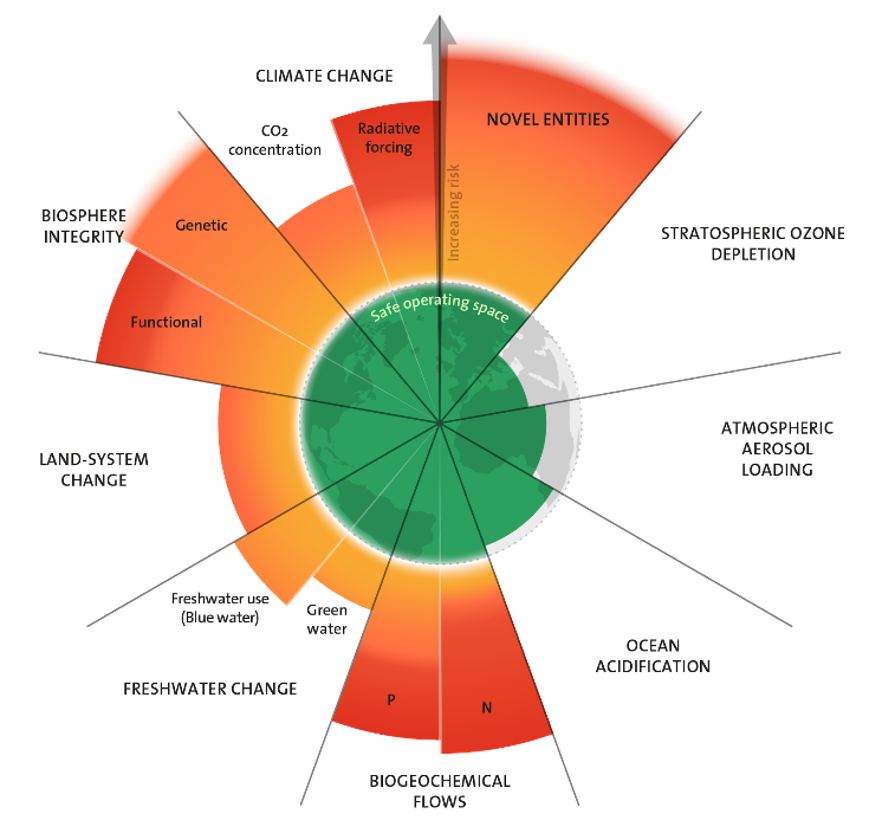
\includegraphics[width=0.58\textwidth]{Figures/fig_01.png}
    \caption{Schematic of the nine Plantary Boundries. (Richardson et al. 2023).}
    \label{fig:introduction_01}
\end{figure}

Thus, humanity stands in front of a challenge in sustaining the supply of animal proteins. Meanwhile, the EAT-Lancet commission declares numerous arguments for a protein shift towards plant-based alternatives. Where human health and environment are two pillar arguments of the diet recommendations (Willett et al., 2019).

\subsection{Aim and Objectives}
The scope of this report narrows down to a nutrient-rich product with low water impact and low CO2  footprint. The formulation targets two of the nine planetary boundaries, freshwater change and CO2-concentration. This report aims to present a hemp protein bar, which served as an alternative to animal-source protein bars, which could help in mitigating the transgression of these planetary boundaries. 

\subsection{Market Trends \& Target Consumer Group}
With animal sourced protein risking straining the planets' resources, a shift in the traditional diet of the Nordic countries has been studied. On the very subject, Geirsdóttir et al. 2023 provided a thorough scoping-review on Nordic Nutrition Recommendations. They concluded that a shift towards a more plant-based protein diet would benefit both health and the environment. Hence, given the need for a shift, the demand for plant-based protein is expected to increase, while the European meat consumption is expected to decline, the consumption still exceeds that of the respective countries' national recommendations (typically 300-500 g/week). (OECD/FAO, 2023) The Smart Protein Project collects data which helps understanding the status and attitude towards a plant-based diet in various European Countries. Among many surveys, it is stated that “Plant-based sweets, meat alternatives, and milk substitutes emerge as the most sought-after categories for expanding plant-based options.” This accounts for 27\% of the cohorts “express for desire” of such product. Among the top 6 drivers for choosing these products, “health” and “environmentally friendly” are mentioned (45\% and 21\% respectively) (ProVeg, 2023). 

\vspace{1em}
Looking at market predictions and current trends, the global growth of plant-based protein supplements is currently outpacing the growth of that animal source. Which yet again correlates with the future need for sustainable plant-based protein (Market.us, 2024). The consumption of such is seen in either ready-to-eat products or supplements as concentrates or isolates. It is shown that nutritious / functional protein bars are an emerging market as in 2023, it was worth 0,92 billion \$ in Europe. Offering a convenient, ready-to-eat alternative to reach fitness goals. The main consumers of such products are found to be Millennials and Generation Z, with enthusiasm over high protein bars (PW, 2024). Hence, targeting younger consumers is of interest. Furthermore, a plant-based protein bar would target any consumer interested in reducing animal consumption, complementing their daily protein intake, and supplementing regular meals.

\subsubsection{Existing Market}
As development of plant-based fitness supplements and ready to eat products are increasingly popular, a wide range of products are available. Below is a showcase of an Estonian and Finnish producer, which specialize in hemp-based products and/or raw material. A showcase of a current hemp bar product is also presented.

\subsubsection*{Nordic Hemp, Estonia}
Specializes in organic industrial hemp growing and processing of raw material. Production of 6000 ha / year. (Nordic Hemp, 2025)
\begin{itemize}
    \item Sorting
    \item Dehulling
    \item Processing
    \item Protein isolation
\end{itemize}

\subsubsection*{Impolan Kasvitila, Finland}
Impola plant farm is a family-owned company in its fourth generation. (Impolan Lasvitila, 2025)
They grow and produce product for end-consumers. 

\begin{minipage}{0.6\textwidth}
    \begin{itemize}
        \item Pet and Feed products
        \item Pressing
        \item Dehulling
        \item Hemp chocolate
        \item Hemp muesli
        \item Hemp meal
    \end{itemize}
    \end{minipage}%
    \hfill
    \begin{minipage}{0.35\textwidth}
        \centering
        
\includegraphics[width=\linewidth]{Figures/fig_02.jpg}
        \captionof{figure}{Hemp protein bar by Nordic Hemp. Selection of products from Impolan Kasvitila, Finland.}
        \label{fig:introduction_02}
    \end{minipage}

\subsubsection*{ROO'bar by Smart Organic, Bulgaria}
Roobar is the flagship brand by Smart Organic AD. They are the largest producer of “minimalistic plant-based bars.” They focus on “... 4-5 ingredients… organic, vegan, raw, and gluten-free”. The production is estimated to 1 million bars per month, and they are accessible in around 50 countries. (Smart Organic, 2025)
\begin{wrapfigure}{r}{0.3\textwidth} 
    \centering
    
\includegraphics[width=\linewidth]{Figures/fig_03.jpg}
    \caption{ROO'bar Hemp protein bar}
    \caption*{Roobar Hemp protein bar}
    \label{fig:introduction_03}
\end{wrapfigure}


\begin{itemize}
    \item Broad range of different bar products
    \item Owner of a wide range of ready to eat brands
\end{itemize}


\begin{wraptable}{l}{0.5\textwidth} 
    \centering
    \caption{Ingredients: Dates, almonds, hemp protein (18\%). Nutrient declaration per 100 g.}
    \label{tab:your_label}
    \begin{tabular}{|l|l|} 
        \hline
        Energy & 1582 kJ/377kcal \\ 
        \hline
        Fat & 11 g \\ 
        \hline
        - Fatty acids & 1.9 g \\ 
        \hline
        Carbohydrates & 49 g \\ 
        \hline
        - Sugars & 33 g \\ 
        \hline
        - Dietary Fibers & 11 g \\ 
        \hline
        Protein & 14 g \\ 
        \hline
        Salt & 0 g \\ 
        \hline
    \end{tabular}
\end{wraptable}


\section{Product Concept}
It is estimated that only 35\% of the globally produced plant protein is consumed by humans. Meanwhile the current market offers a wide range of plant-based proteins available which are well fitted for human consumption. Common choices include formulations with oat, wheat, hemp, soy and pea to name a few (Gorissen et al., 2018). The Cannabis sativa L., a Cannabaceae known as ‘‘hemp’’ is of increasing interest because it is highlighted as an environmentally friendly and economically high-potential crop. Its history as a source for medicine, fiber and food dates back 6000 years, and the cultivation of hemp with close to no levels of tetrahydrocannabinol (THC), the psychoactive compound found in cannabis, has increased to use in foods since strains with a THC content below 0.3\% was approved in EU in 1996. Among its many advantages are fast growth and low dependency on pesticides, which benefits biodiversity and healthy soils. Furthermore, its seeds provide a valuable source of nutrients. (Chapter 6 Industrial Hemp Seed). Globally, the trend of increasing interest for hemp seeds is clear, as the production increased from 2,718 tons to 5,449 tons between 2015 and 2020. 

\begin{table}[h] 
    \centering
    \caption{Ingredients: Dates, almonds, hemp protein (18\%). Nutrient declaration per 100 g.}
    \label{tab:your_label}
    \begin{tabular}{|l|l|} 
        \hline
        Energy & 1582 kJ/377kcal \\ 
        \hline
        Fat & 11 g \\ 
        \hline
        - Fatty acids & 1.9 g \\ 
        \hline
        Carbohydrates & 49 g \\ 
        \hline
        - Sugars & 33 g \\ 
        \hline
        - Dietary Fibers & 11 g \\ 
        \hline
        Protein & 14 g \\ 
        \hline
        Salt & 0 g \\ 
        \hline
    \end{tabular}
\end{table}

\vspace{1em}
Thus, developing a convenient hemp-based bar would harness the many benefits of the not-so-novel ingredient that is hemp seed. Below is a mock up of the Hemp Protein Bar (figure 4).

\begin{figure}[H]
    \centering
    \includegraphics[width=0.54\linewidth]{Figures/fig_prod_concept_01.png}
    \caption{AI-generated illustration of a medieval marketplace. Generated using DALL·E 3 (OpenAI, 2025) with the prompt: "Mock up of a hemp bar picture half coved in chocolate ".}
    \label{fig:prod_concept_01}
\end{figure}


\subsection{Macronutrients in Hemp Seeds}
Hemp seeds typically contain around 20-30\% protein, 25\%-35\% lipids, 20-30\% carbohydrates and 4-7\% of ash (Figure 5). It has a balanced composition with particularly low starch content. (Montero et al 2023) 

\begin{figure}[H]
    \centering
    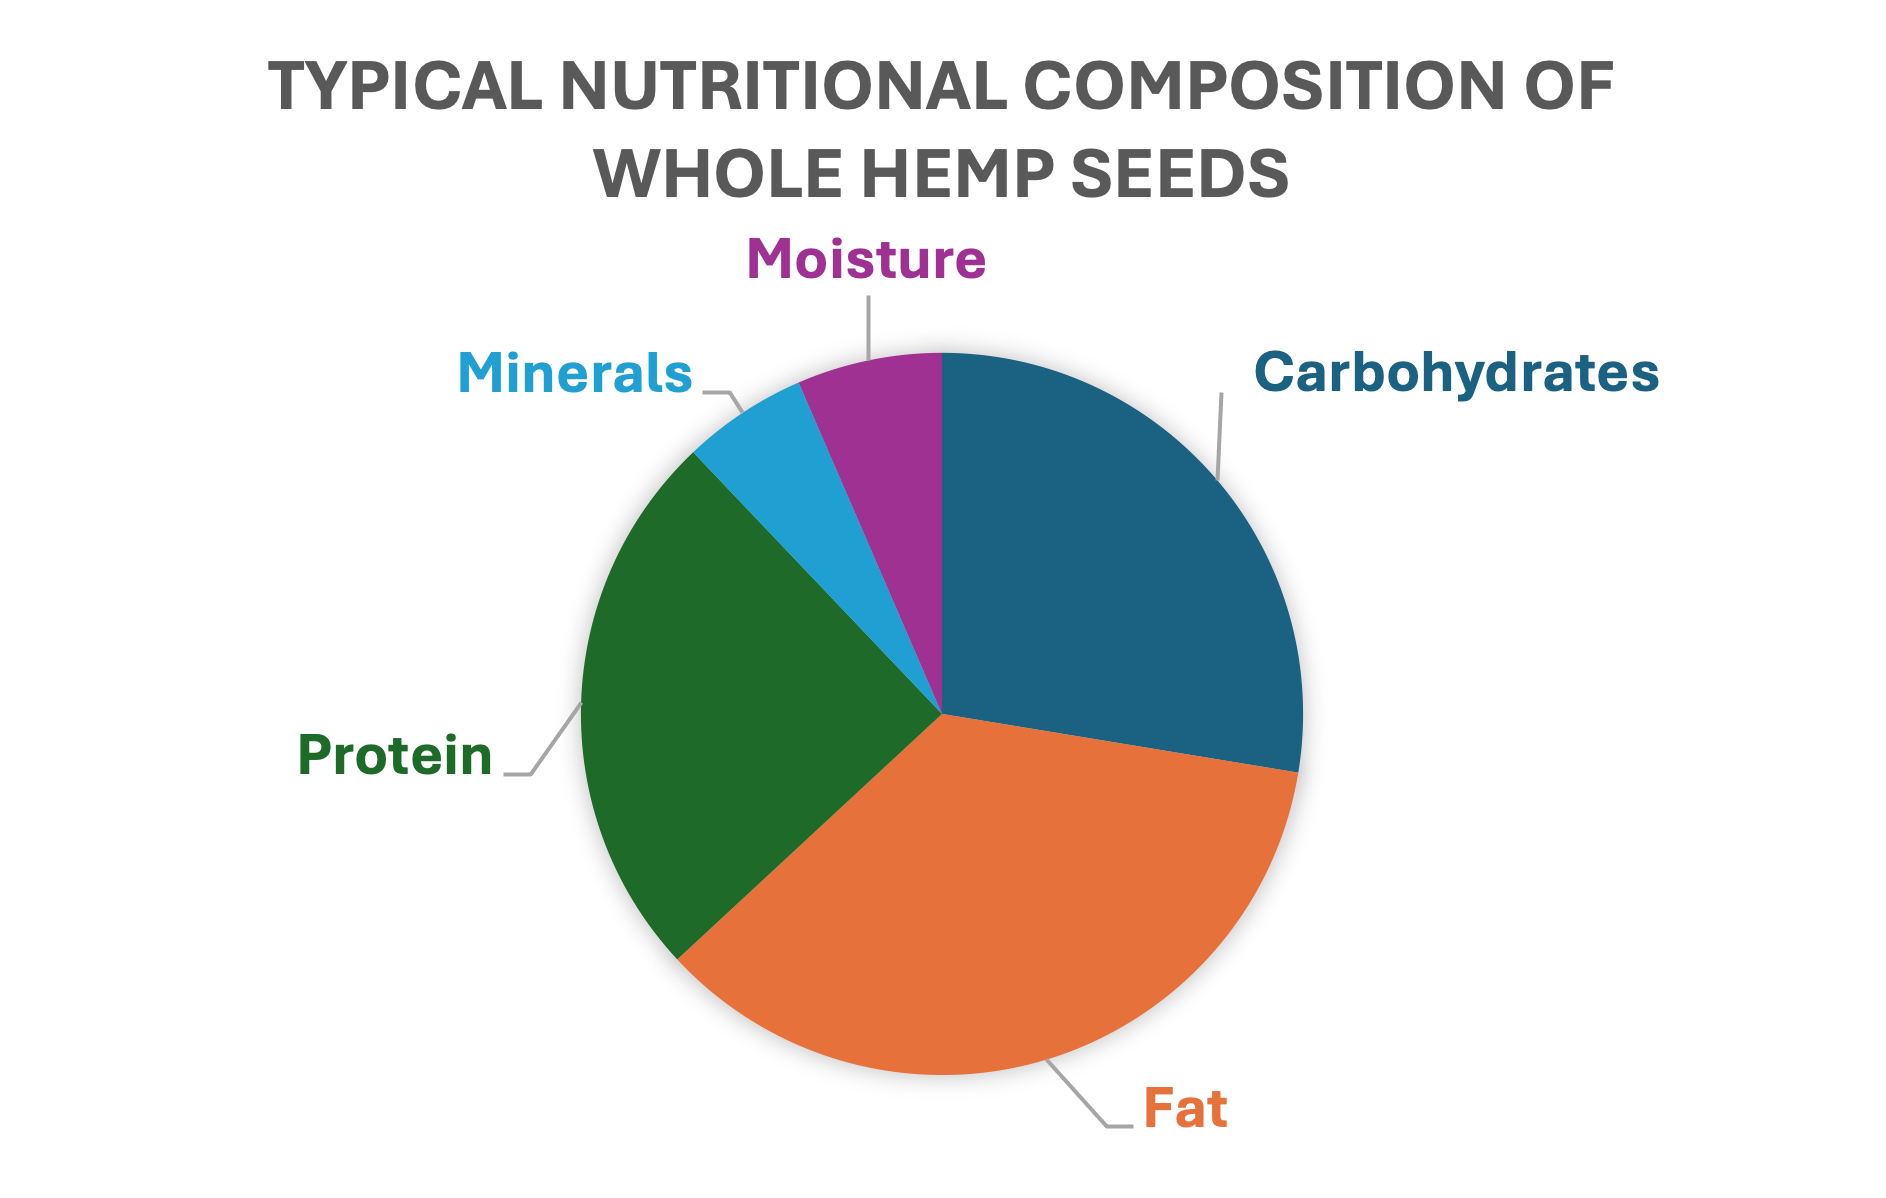
\includegraphics[width=0.75\linewidth]{Figures/fig_prod_concept_02.png}
    \caption{Composition diagram of whole hemp seeds}
    \label{fig:prod_concept_02}
\end{figure}

\subsubsection{Protein}
Hemp seeds are an excellent source of high-quality protein, typically containing 20–30\% protein, with dehulled hemp seeds having even higher protein contents, ranging from 30\% to 38\%. (chapter 4 hemp seed book). The two main proteins in hemp seeds are albumin (33\%) and edistin (65\%), which have very similar structures to plasma proteins which helps the digestibility in humans. Hemp seeds provide a complete amino acid profile, containing all nine essential amino acids required by humans, making them comparable to other high-quality proteins like egg white and soybeans (Chapter 10). 

\vspace{1em}
The protein is also particularly rich in arginine, glutamic acid, and aspartic acid, where arginine is especially valuable as it is a precursor to nitric oxide, which enhances blood flow and helps maintain normal blood pressure, contributing to cardiovascular health (chapter 11 hemp book)
Hemp proteins are highly digestible, with dehulled hemp seeds demonstrating superior protein digestibility (83.5–92.1\%) (hemp nutritional value). This is partly attributed to the absence of protease inhibitors in hemp seeds (Hemp seed bioactivity). 

\vspace{1em}
A study has analysed the macronutrient composition and protein quality of 30 hemp seed products from Western Canada, including whole seeds, dehulled seeds, and hemp seed meal. Crude protein, fat, and amino acid profiles were determined, and protein quality was assessed using the Protein Digestibility-Corrected Amino Acid Score (PDCAAS) method, based on a rat bioassay and FAO/WHO amino acid requirements for young children. Average protein content ranged from 24.0\% in whole seeds to 40.7\% in hemp seed meal. Protein digestibility was 84–98\%, with protein digestibility-corrected amino acid score (PDCAAS) values of 46–66\%, highest in dehulled seeds. The protein digestibility-corrected amino acid score of dehulled hemp seed is comparable to lentils and is about half that of casein, and almost twice that of almonds (chapter 10 hemp seed book)

\subsubsection{Fatty Acids}
Hemp seed oil is primarily composed of polyunsaturated fatty acids, PUFA (over 80\%) including fatty acids like essential linoleic acid (omega-6) and alpha-linolenic acid (omega-3). (Chapter 10 hemp seed book) Dehulled hempseeds have a healthy balance of omega-6 to omega-3 polyunsaturated fatty acids (2.5:1) (Chapter 1 hemp book)

\vspace{1em}
Unsaturated fatty acids help protect against cardiovascular disease, obesity, diabetes, and inflammation. EFSA recommends an optimal omega-6/omega-3 ratio of 3:1 to 5:1. Hemp seed oil typically shows a ratio of 2.5–3.5:1, which is a desirable range linked to lower chronic disease risk. (Hemp nutritional value pdf)

\subsubsection{Carbohydrates}
About 98\% of the carbohydrates in hemp seeds are dietary fiber, mainly insoluble dietary fibers (80\%), such as cellulose, lignin and hemicellulose. Dietary fiber resists enzymatic digestion in the small intestine and undergoes partial or complete fermentation in the large intestine. The remainder of the carbohydrates in hemp seeds is starch. Therefore, hemp seeds are considered a low-starch food and an excellent source of dietary fiber. (Hemp nutritional value pdf) 

\vspace{1em}
The dietary fibers from hemp seeds are associated with positive effects on the digestive tract support by acting as prebiotics. The fermentation of fibers in the colon generates short-chain fatty acids that have beneficial roles in the body. (Hemp seed bioactivity pdf). In the Western countries the consumption of dietary fiber is lower than the recommended intake, making hemp seeds an attractive ingredient to meet the recommended daily intake of dietary. However, processing might affect the amounts of dietary fibers in hemp seeds. 

\subsection{Micronutrients: Vitamins and Minerals}
Hemp seeds are rich in vitamins and minerals. Just 50 mg of hemp seed can supply at least half of the recommended daily allowance of copper, magnesium, and zinc, and exceed the recommended daily allowance of the vitamins A, D, and E. (Chapter 1 hemp book) Hemp seeds also contain other micronutrients such as phosphorus, potassium, calcium, sodium, iron, and manganese. (Chapter 4 hemp book). Hemp seed oil contains fat-soluble vitamins, in particular vitamin E (tocopherols) and vitamin A which respectively has an antioxidant role and is beneficial for skin integrity and Vitamin D is important for bone health and the immune system (Hemp nutritional value pdf)

\vspace{1em}
Besides the macro- and micronutrients, secondary metabolites, such as terpenes, phytosterols and flavonoids, constitute essential components of the defence response of the hemp plant to biotic and abiotic stresses. However, the composition of these secondary metabolites can be influenced by cultivation conditions, providing a distinct fingerprint of different production regions. It is suggested that these compounds contribute with antioxidative, antimicrobial, and anti-inflammatory properties in the human body. Phytosterols for instance, are not synthesized in humans, but can when ingested from plants, reduce cholesterol levels in the human body by changing the cholesterol solubility in the intestine. (Tănase et al. 2024).

\subsection{Potential Side Streams}
The industrial hemp plant has a versatile plant body which consists of seeds, leaves, stem, and flowers with several application opportunities depending on the part of the plant. Particularly the stem is a valuable source to produce hemp fiber which can be used for rope, building materials, paper, or textiles. The seeds, dehulled or whole, can be utilized as a food source. The hemp flower can be used to produce cosmetic and pharmaceutical products, including essential oils. When looking further into hemp as a natural source to bast fiber a life cycle assessment reveals that hemp performs better than glass fiber by weight and compared to cotton, hemp requires less water and pesticides to grow although hemp fiber is known to be coarser and stiffer than cotton which has a softer appearance. (Kaur \& Kander 2023). 

\vspace{1em}
When processing the stem to hemp fiber a by-product of shives is made. It can be used to produce hemp concrete which is a bio-composite and carbon-negative alternative to concrete for construction and insulation. (Yano \& Fu 2023). These useful side streams make hemp even more attractive to use as an ingredient in foods. 

\subsection{Dietary Pattern of the Chosen Consumer Group and Product Fit}
Our hemp seed bar is uniquely positioned to seamlessly integrate into several contemporary dietary patterns, directly addressing the needs and preferences of our diverse target consumer groups within the Millennial and Generation Z age group.

\vspace{1em}
For vegetarians and vegans dehulled hemp seeds are an excellent source of high-quality, plant-based protein. The seeds naturally contain all nine essential amino acids required by humans, offering a complete protein profile that can be challenging to obtain from other plant sources. (Chapter 1 hemp seed book) The protein in dehulled hemp seeds also boasts superior digestibility (83.5\%-92.1\%) compared to whole hemp seeds and hemp meal, making its nutrients more accessible. They also provide a healthy balance of omega-6 to omega-3 polyunsaturated fatty acids (typically 2.5:1 to 3.5:1), which is desirable for overall human nutrition. (Hemp nutritional value pdf) Hemp protein and flour can serve as an alternative for soy ingredients (Chemical composition and biological activities of PDF) 

\vspace{1em}
A health-conscious person or athlete would also use it for its excellent source of protein, especially because of the high value protein composition with the nine essential amino acids. Furthermore, it scores high in terms of digestibility which makes our bar effective for muscle recovery and satiety. (Chapter 10 hemp book) Many athletes need to have control on their calorie needs. Our bar could therefore be an easy boost of calories or be used as a substitute for a snack or meal.
\vspace{0.5em}
The bar is rich in healthy fats, including the beneficial omega-6 to omega-3 ratio, which is important for cardiovascular health and may help prevent chronic diseases. (Hemp nutritional value pdf)

\vspace{1em}
Our bar is also a good source of essential minerals like copper, magnesium, and zinc, and provide vitamins A, D, and E, which also talks to the health-conscious person (Chapter 1 hemp book)

\vspace{1em}
For individuals with dietary restrictions and/or allergies our bar is also a great option, as our bar is naturally gluten-free, making it a safe nutritious option for people with celiac disease or gluten sensitivities. (Chapter 1 hemp book) Hemp proteins are generally considered to have low allergenicity compared to common proteins like soy, dairy, or wheat, broadening its appeal for those with various food allergies. (Chapter 11 hemp book \& Hemp nutritional value pdf)

\vspace{1em}
For environmentally aware consumers our hemp-based product directly supports environmental sustainability due to it having a low environmental impact, actively contributing to improved soil health, water quality, have carbon-negative crops and requiring no or little pesticide use. (Chapter 1 hemp book \& hemp nutritional value PDF \& hemp seed bioactivity) 

\vspace{1em}
The pre-packaged protein bar format offers convenience and time efficiency, requiring no preparation or cleanup for the people on-the-go. It delivers the balanced nutrition derived from dehulled hemp seeds in an easily consumable form, perfectly fitting the needs of busy individuals seeking healthy and convenient dietary options.


\section{Formulation and Raw Materials}
The formulation of the hemp seed bar is an important factor, as it regulates the final nutritional composition and determines the parameters for the upstream and downstream processing steps. Using consistent suppliers and high-quality raw materials are key factors in maintaining a predictable, consistent production. Production as such would decrease faults, which reduces waste and ensures safe a safe high-end product to the final consumer. 

\vspace{1em}
Given the lack of sweetness of hemp seeds, the bar is formulated with naturally sweet components such as dried dates and agave sirup. Along with a caramelly flavor, important cohesiveness of the bar is achieved. The dates are dried which reduces water content and thus increases sugar concentration and intensifies flavor. Minimum processing other than dehydration and pitting ensures valuable components such as micronutrients and fibers are included.

\vspace{1em}
To complement the protein value (which lacks in lysine), potato protein isolate is used. During its production, it undergoes heavy processing which concentrates the protein content while reducing other macronutrients, minerals and vitamins (Wagley et al., 2019).

\vspace{1em}
Rolled oats are used as a structural component. It is chosen as it is a gluten free, cheap, readily available raw material known to consumers. It undergoes dehulling, rolling and steaming, which maintains the high fiber content while inactivating lipase enzymes to prevent oxidation and extend shelf life (Ekelund et al., 2024). Ground flax seeds are also included to account for the loss of dietary fibers in Hemp. The flax seeds are grounded to inhibit toxic effects of cyanogenic glycosides (Nowak et al., 2023).

\vspace{1em}
Preprocessing of hemp seeds aims to partially remove the hull/husk (figure 6). The macronutrient profile of the seed is significantly affected by the processing method. Although the formulation does not involve hemp protein isolate, HPI, many studies on this subject point at the effects of preprocessing. 

\vspace{1em}
For example, a study by House et al., 2010 evaluated HPI derived from whole seeds, hemp seed meal, and solely hulls. The study could show that the amino acid composition is different among the three processed raw materials. In the works by Shen et al., 2020 the HPI of dehulled and whole seeds were comprehensively investigated in terms of aromatic components, colour, and protein characterization. Dehulled seeds would increase the extraction yield by 21.52 \% and protein recovery yield (46.90\%) of the HPI. Naturally, the HPI with whole seeds would contain increased amounts of lipids and carbohydrates. The preprocessing also had a profound impact on colour, were whole seeds generated a darker coloured HPI. This matter is further explained in the section “4.1 Effects on Processing”

\vspace{1em}
Vanilla extract, cocoa and sea salt are used to characterize the aroma of the bar. Potentially masking some of the earthy off-flavours from the other ingredients. 


\begin{figure}[h]
    \centering
    \begin{subfigure}{0.45\textwidth}
        \centering
        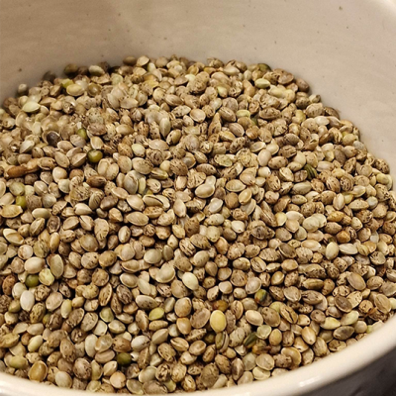
\includegraphics[width=\linewidth]{Figures/fig_formulation_06.png}
        \caption{Whole hemp seeds}
        \label{fig:whole_hemp}
    \end{subfigure}
    \hfill
    \begin{subfigure}{0.45\textwidth}
        \centering
        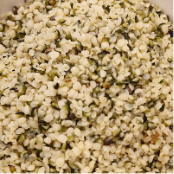
\includegraphics[width=\linewidth]{Figures/fig_formulation_06.1.png}
        \caption{Dehulled hemp seeds}
        \label{fig:dehulled_hemp}
    \end{subfigure}
    \caption{Whole and dehulled hemp seeds (Svensk Hampaindustri, 2025).}
    \label{fig:whole_dehulled}
\end{figure}


\section{Processing and Manufacturing}
The production process of the protein bar can be seen on Figure 7.
\begin{figure}[H]
    \centering
    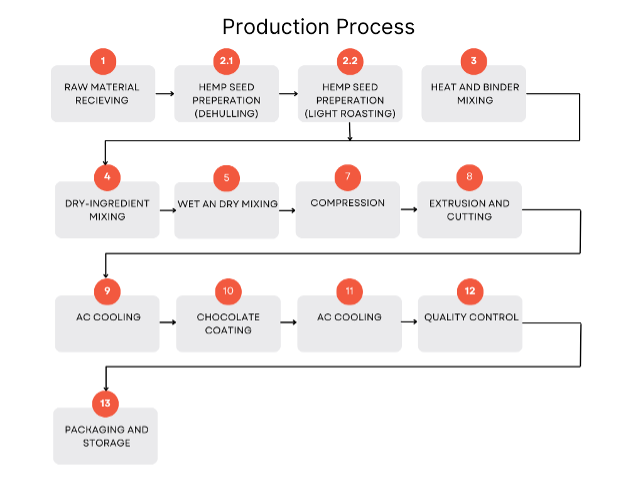
\includegraphics[width=0.8\textwidth]{Figures/fig_process_01.png}
    \caption{A flowchart with a visualization of the production process of the hemp protein bar}
    \label{fig:process_flow_diagram}
\end{figure}

\textit{Sourcing and preparing} raw materials – all ingredients are inspected for quality and stored under appropriate conditions to maintain freshness. All ingredients are weighed and portioned accurately according to the recipe formulation, ensuring batch-to-batch uniformity. This ensures that only safe, high-quality, and properly measured ingredients enter the mixing stage, laying the foundation for a consistent protein bar in terms of flavor, texture, and nutritional profile.

\vspace{1em}
\textit{Dehulling hemp seed} – Increases absorption of proteins and nutrients.

\vspace{1em}
\textit{Light roasting} – of the dehulled hemp seed (75°C-80°C) - improves digestibility, and reduces anti-nutritional factors and lower microbial load.

\vspace{1em}
\textit{Mixing} to homogeneous mixture – evenly distributed throughout the mixture providing a consistent texture and flavor in every bar. Time and temperature in mixing are controlled to ensure that every batch is consistent.

\vspace{1em}
\textit{Compression} – shaping the mixture into a form that is suitable for further processing. Using large presses ensures a uniform sheet, which helps create consistency in texture and flavor throughout the bar.

\vspace{1em}
\textit{Extrusion and cutting} – A combination of extrusion and cutting technologies are used to shape the mixtures into bars. The extrusion process forces the mixture through a die, after which a knife cuts the long bars into the desired length.

\vspace{1em}
\textit{AC cooling} – is used to ensure that the bar maintains the desired temperature throughout the process, as mixing and pressure from extrusion can increase the temperature of the product.

\vspace{1em}
\textit{Chocolate coating} – for flavour.

\vspace{1em}
\textit{AC cooling} – to solidify the chocolate.

\vspace{1em}
\textit{Quality control} – Both automated sensors and visual inspection for defects or foreign objects. Taking samples to ensure that our product meets quality standards, as well as for example checking that the product contains enough protein to be claimed as a product with a high protein content. 

\vspace{1em}
\textit{Packaging} – wrap each bar individually and in a material that keeps the protein bar safe and to ensure that the bar does not undergo oxygenation and to preserve freshness. This process also includes labelling and coding to ensure traceability and compliance with regulatory requirements.

\subsection{Effects on Processing}
Hemp seeds contain several antinutritional, such as phytic acid, tannins and saponins. The presence of tannins and saponins can reduce the bioavailability of nutrients and disrupt both metabolism and digestive functions (kapitel 4 hampbog). The presence of phytic acid can lead to mineral deficiencies (e.g. iron, zinc and calcium), as it can inhibit the absorption of these. (kapitel 10 hampbog). Polyphenols, of which tannins are a part, are often found in the shell of hemp seeds (hemp nutritional value pdf). The same applies to phytic acid. Studies have shown that there is significantly more phytic acid present in whole hemp seeds 3.5 g/100g compared to 2.1 g/100g in hulled hemp seeds. That is a reduction of 40\%. (kapitel 4 hampbog).

\vspace{1em}
According to House et al. (2010), whole hemp seeds have a protein digestibility of approximately 84–86\% and a protein digestibility-corrected amino acid score (PDCAAS) value of 49–53\%, while dehulled hemp seeds reach a digestibility of 91–97\% and a PDCAAS value of 63–66\%. This improvement is primarily due to the fact that the hull contains a large part of the fiber fraction of the seed, which inhibits digestibility, so when the hull is removed, the fiber content is significantly reduced, making the protein more available and thus improving the overall protein assessment (PDCAAS) (Evaluating the Quality of Protein from Hemp Seed pdf.) Therefore, by using a majority of dehulled hemp seeds instead of whole hemp seeds, we reduce the content of antinutrients and increase the nutritional quality of the protein.

\vspace{1em}
Plant proteins naturally contain antinutritional factors such as trypsin inhibitors, glucosinolates, phenols and phytates, together with a high content of dietary fiber, which can negatively affect protein and amino acid digestibility and bioavailability. Heat processing can effectively help to remove or reduce these compounds, leading to higher protein digestibility. However, high heat treatment can have negative effects as it can affect the chemical transformations of amino acids. Some amino acids, such as lysine, can be chemically transformed and become unavailable during heat treatment or other severe processes, leading to problems such as the formation of Maillard reaction products. This underlines the need for appropriate processing conditions to avoid such. (Protein Quality Report No 92 web version .pdf)



\begin{table}[h]
    \centering
    \caption{Protein digestibility-corrected amino acid scores of hemp protein sources in comparison to other food proteins. (Evaluating the Quality of Protein from Hemp Seed pdf.)}
    \label{tab:process_table_01}
    \begin{tabular}{l c}
    \hline
    \textbf{Protein source} & \textbf{PDCAAS (\%)} \\
    \hline
    Casein               & 100 \\
    Egg white            & 100 \\
    Beef                 & 92  \\
    Soy protein isolate  & 92  \\
    Chickpeas (canned)   & 71  \\
    Pea flour            & 69  \\
    Kidney beans (canned)& 68  \\
    Dehulled hemp seed   & 61  \\
    Pinto beans (canned) & 57  \\
    Rolled oats          & 57  \\
    Lentils (canned)     & 52  \\
    Hemp seed            & 51  \\
    Hemp seed meal       & 48  \\
    Whole wheat          & 40  \\
    Almond               & 23  \\
    \hline
    \end{tabular}
\end{table}

\vspace{1em}
At the same time, a study has shown that hemp protein isolates improved proteolysis when heated at 75 °C and 80 °C, but already at 90 °C it caused reduced proteolysis. (hemp seed bioactivity pdf) Therefore, we have chosen to lightly roast our dehulled hemp seeds to achieve the highest possible protein absorption, but with an eye not to reach too high a temperature, as we want to avoid a greater loss of lysine and reduced proteolysis.


\section{Final Nutritional Profile of the Bar - Lucas}
\subsection{Nutritional Composition Overview}
In this section of the report, the macronutrient composition of the hemp seed protein bar is examined, namely protein, dietary fibre, and fatty acids. The final nutritional profile was estimated based on the formulation and calculated contributions of each ingredient. Table 6 shows the magnitude of each ingredient in the bar, where the highlighted cells represent the top contributors that will be examined in greater detail. This section further outlines the amino acid and fatty acid spectrum, evaluates potential nutrition and health claims considering EU regulations and EFSA opinions, and compares the bar’s profile to existing market products.



    \begin{table}[t]
        \caption{The table indicates the 10 ingredients that the product is made of, and the respective values for three of the most notable macronutrients and moisture content. The top five contributor for each of the factors is highlighted in green, ranging from dark to light-green from highest to lowest value corresponding to the amount of the macronutrient in the bar. }
    \label{tab:df_amino_acids_01}
    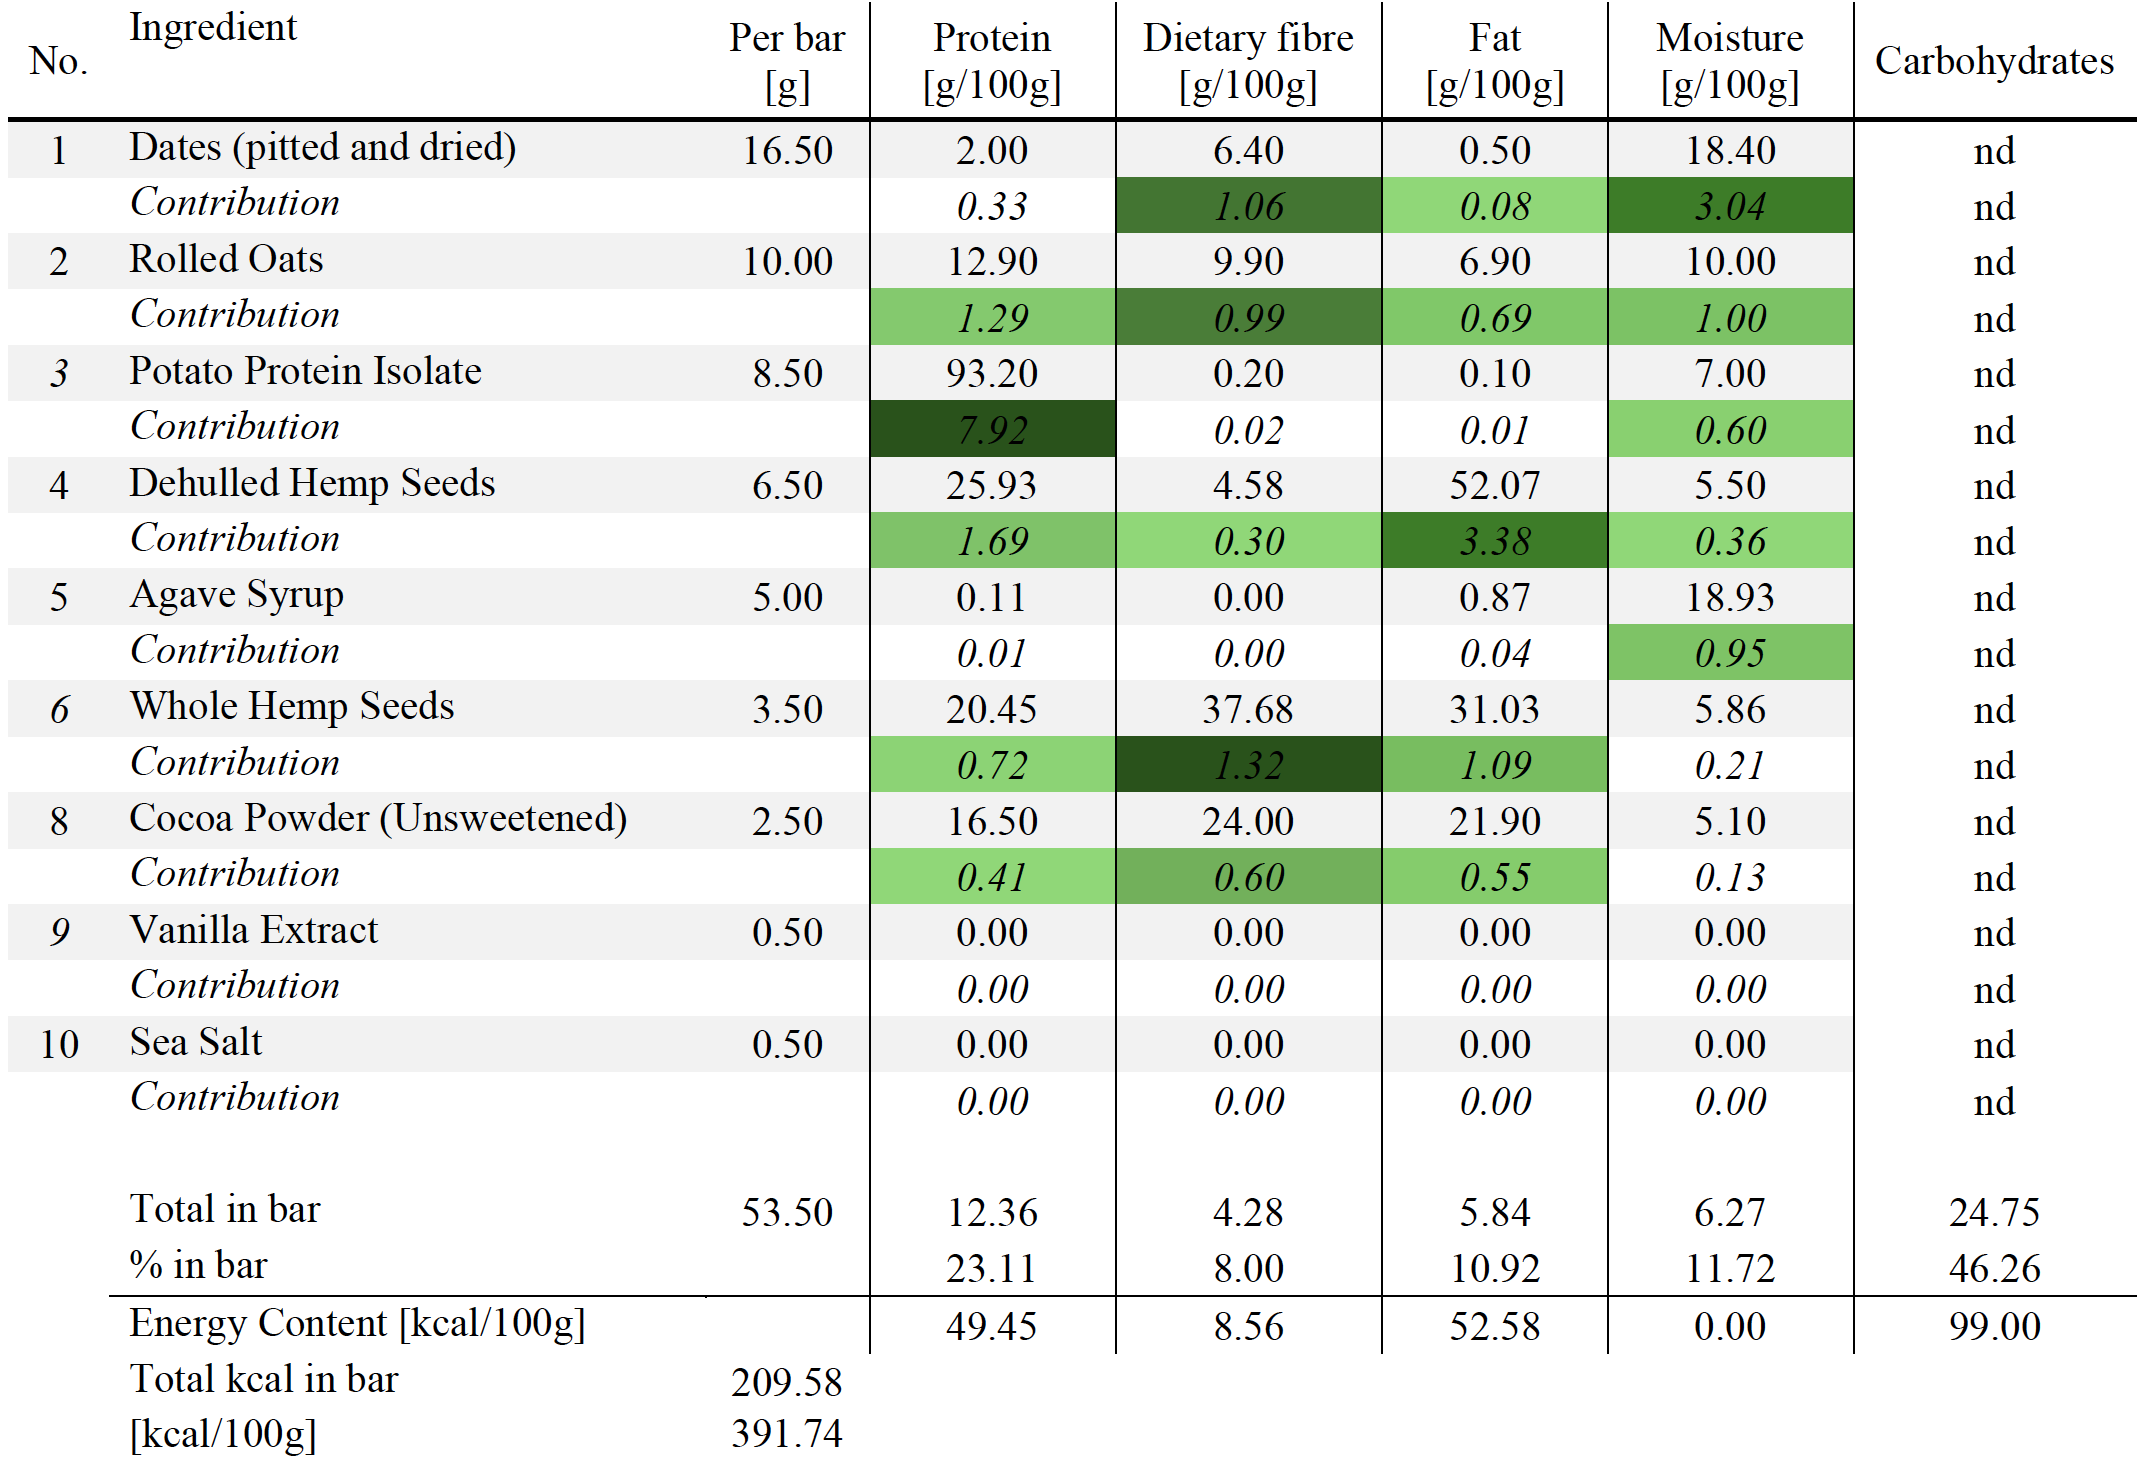
\includegraphics[width=\linewidth]{Figures/tab_overall_ingredients_01.png}
\end{table}

\subsection{Macronutrient Composition}
As shown in Table 6, the hemp seed protein bar delivers 209.6 kcal per 53.5 g bar, with a macronutrient profile characterised by 12.36 g protein, 4.28 g dietary fibre, 5.84 g fat, 6.27 g moisture, and 24.75 g carbohydrates. This balance between protein, fibre, and healthy fats underlines the bar’s potential as a nutrient-dense snack.

\vspace{1em}
The overall macronutrient profile was calculated using data from various sources to determine the contribution of each ingredient. For each raw material, published nutrient values were combined with the amount used per bar (g) to estimate the contribution of the respective ingredient. The calculations followed Equation 5.1. 


\begin{equation}
    \text{Contribution [g]} = 
    \frac{\text{Nutrient content [g/100g]} \times \text{Ingredient weight [g]}}{100}
    \label{eq:contribution}
\end{equation}

This approach was applied for protein, dietary fibre, fat and moisture. Carbohydrates were excluded from direct analysis, thus their content was derived by calculating the difference, as outlined in Equation 5.2. 

\begin{equation}
    \text{Carbohydrates [g]} = 
    \text{Total weight [g]} - (\text{Protein} + \text{Fat} + \text{Dietary fibre} + \text{Moisture})
    \label{eq:carbohydrates}
\end{equation}

The energy content of the bar was subsequently estimated while adhering to the conversions factors defined in regulation (EU) no. 1169/2011 (protein 4 kcal/g, carbohydrates 4 kcal/g, fibre 2 kcal/g) \cite*{art_17}. The energy content for moisture was assumed to contribute with 0 kcal/g, thus neglected in the calculations. 

\vspace{1em}
Based on published nutrient values and the calculations described, the bar (53.5 g) provides 209.6 kcal, equivalent to 391.7 kcal/100 g. Its macronutrient composition - 23.1\% protein, 8.0\% dietary fibre, and 10.9\% fat - qualifies the product for the nutrition claims, “High protein” and “High fibre.” These claims comply with the conditions defined in the Annex of Regulation (EC) No 1924/2006, which governs nutrition and health claims across the European Union \cite*{art_16}.    

\subsubsection{Protein Content and Quality}
Protein intake is essential for muscle protein synthesis, but the source and type of protein substantially influences its digestibility and utilisation. Since humans cannot synthesise essential amino acids, these must be obtained through diet. Consequently, the overall protein composition, and particularly the essential amino acids profile, is a key to determine protein quality \cite*{art_08_protein_amino}.

\vspace{1em}
The hemp seed protein bar provides a total of 12.36 g protein per bar. As shown in Table 6, the main contributors for protein are potato protein isolate, rolled oats and dehulled hemp seeds. Dehulling is a processing step which has a significant effect on protein quality. It improves digestibility and reduces antinutritional factors, while also elevating the protein fraction of the hemp seed \cite*{HempBook}. To further characterise the protein profile, Table 3 presents an in-depth analysis of the protein composition, with respect to each ingredient’s amino acid composition. The data was compiled from multiple sources, yet the methodologies used for amino acid determination has been similar across the studies \cite*{art_08_protein_amino, frida_food, art_09_potato_protein, art_10_hemp_aa}.

\vspace{1em}
The amino acid profile derived from the three main protein contributors includes all nine essential amino acids, confirming the bar as a complete protein source for the consumer. In each of the three main protein contributors, Leucine is the most abundant essential amino acid. Overall, Leucine makes up 5.32\% of the total amino acids contributed by the three ingredients. The combined amount of essential amino acids, derived from these contributors, amounts to 2568.83mg, of which Leucine alone constitutes 22.54\%.

\vspace{1em}
For both rolled oats, and dehulled hemps seeds, the lowest contribution stems from Tryptophan. General consensus, regarding the hemp seed amino acid profile identifies Lysine as the limiting essential amino acid. However, published values vary considerably depending on the analytical methods used, cultivation conditions and cultivar \cite*{HempBook}. 

\vspace{1em}
Conversely, Tryptophan was not identified in published data for potato protein isolate, suggesting a scarce amounts present. For this ingredient, Methionine and Histidine was reported as the limiting essential amino acids, only contributing with 1300 mg/100g, which is substantially lower than the levels of the other essential amino acids. 

\vspace{1em}
The hemp seed protein bar exhibits an overall balanced essential amino acid profile, with only Tryptophan contributing under 1\% of the total amino acids, largely due to the absence of reported values in the potato protein isolate. The combination of the three main protein contributors therefore provides an amino acid profile, that can support several potential health benefits. In dehulled hemp seeds, Leucine, Phenylalanine, and Valine are three most abundant essential amino acids. Of these, only Valine is the only one not shared by the top three essential amino acid contributors in potato protein isolate. 

\vspace{1em}
Valine is one of the branched-chain amino acids (BCAAs), together with Isoleucine and leucine \cite*{art_18_valine}. Elevated levels of Valine have been associated with various proposed benefits including improved weight gain, weight gain ratio, enhanced intestinal morphology, strengthened immune responses and increased bone density and strength \cite*{art_19_valine_broiler}. As an essential amino acid, sufficient dietary intake is important, since valine is directly associated with protein synthesis and functions as a glucogenic amino acid within energy metabolism \cite*{art_19_valine_broiler}. Although, valine itself has not been authorised any specific health claims under EU law, protein as a whole is recognised by EFSA to contribute to the maintenance and growth of muscle mass \cite*{art_20_regulation4322012}.

\vspace{1em}
The combination of potato protein isolate, rolled oats, and dehulled hemp seeds enhances the amino acid profile, positioning the hemp protein bar as a sustainable and nutritionally valuable alternative to other conventional protein bars on the market. In addition, the presence of bioactive amino acids supports the bar’s functional value, making hemp a promising ingredient, as a source for high-quality plant protein.
    
\subsubsection{Dietary Fibre Content} 
Dietary fibres are carbohydrate polymers that cannot be absorbed in the human small intestine. These polymers, which contains three or more monomer units, have shown positive potential health benefits with significant prospect of improving carbohydrate metabolism and reducing cholesterol levels \cite*{art_12_df_oats_01,art_13_df_oats_02}. In addition, certain dietary fibre factions act as prebiotics, and has shown physiological beneficial effects by supporting colonic fermentation and short-chain-fatty acids \cite*{art_13_df_oats_02,art_14_df_hemp}. 

\vspace{1em}
The hemp seed protein bar provides a total of 4.28 g dietary fibre per bar. This corresponds to 8 g/100g which exceeds the conditions specified in the Annex of Regulation (EX) No. 1924/2006, for allowing a product to be labelled as “high fibre”.

% Is actually for the section above, but for layout reasons it has been inserted here.
\begin{table}[H]
    \caption{Amino acid composition of the three main protein-contributing ingredients in the hemp seed protein bar (rolled oats, potato protein isolate, and dehulled hemp seeds). The light orange rows indicate essential amino acids (EAAs). Within each amino acid column, the green shading represents relative contribution, ranging from light green (third highest contributor) to dark green (highest contributor). Red cells highlight the lowest contributing ingredient for that specific amino acid.}
\label{tab:df_amino_acids_01}
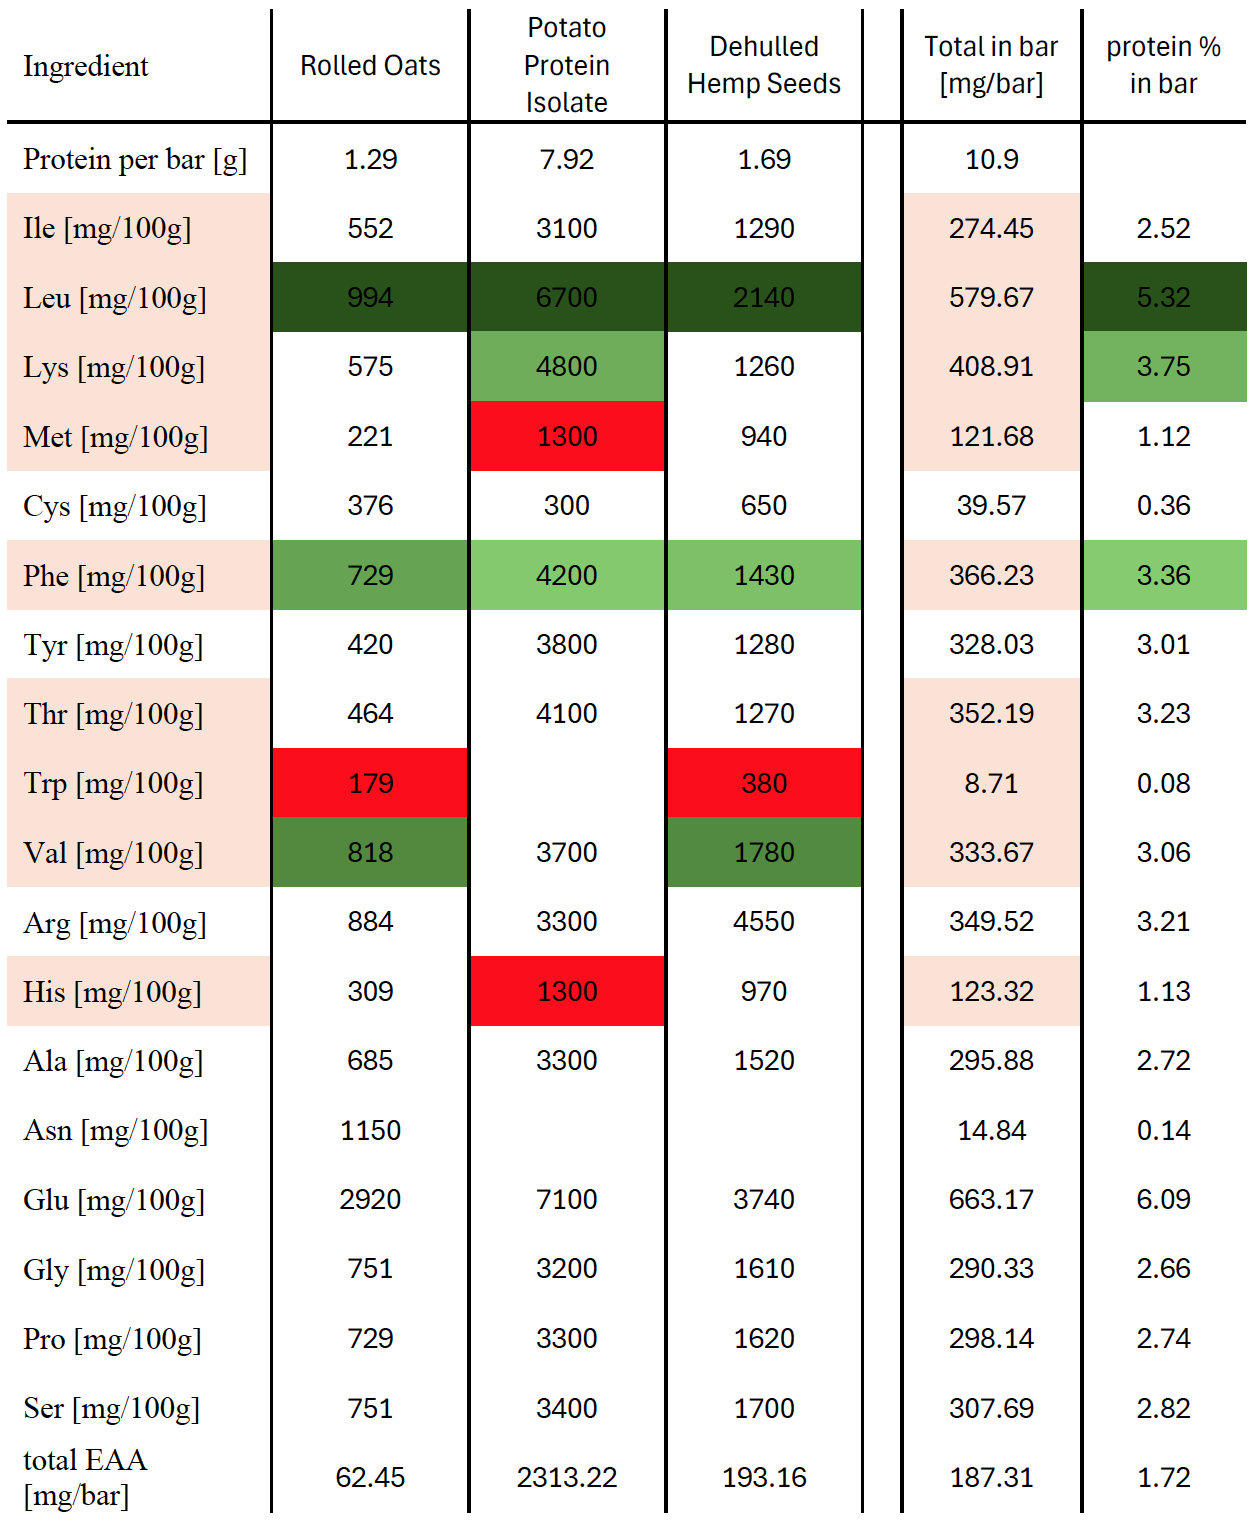
\includegraphics[width=\linewidth]{Figures/tab_amino_acid_01.png}
\end{table}

\vspace{1em}
As shown in Table 6, the main dietary fibre contributors of the hemp seed protein bar are whole hemp seeds, dates (pitted), and rolled oats, who each contributes with 1.32 g, 1.06 g, and 0.99 g, respectively. Processing also influences the dietary fibre profile of the ingredients. In oats, kilning has been used to inactivate lipase enzymes \cite*{art_24_oat_kilning}, drying dates concentrates their fibre fractions while using whole hemp seeds (un-hulled) preserves their full dietary fibre content. Together, these three ingredients provide the majority of the dietary fibre in the product. When compared with the relative proportions in the product (Table 4), it can be noted, that whole hemp seeds, despite representing only 6.54\% of the bar’s weight, contributes the largest share of the total dietary fibre. Conversely, dates and rolled oats, which consist of 30.84\% and 18.69\% of the bar, respectively, provide less fibre relative to their much larger share of the formulation.

\vspace{1em}
Table 4 contains several blank entries, reflecting that not all ingredients contribute to each of the listed dietary fibre type, and that published data remain scarce, particularly for whole hemp seeds. Nevertheless, it is noteworthy that whole hemp seeds consistently display higher values g/100g for their respective fibre fractions. This highlights the role for whole hemp seeds as the most fibre-dense ingredient and the main contributor to the label “high fibre”. 

\vspace{1em}
The three main ingredients providing dietary fibres, contribute with a diverse palette of fibres. Whole hemp seeds mainly contribute with insoluble fibres such as cellulose, lignin, and hemicellulose. Rolled oats supply cellulose + $\beta-glucan$, lignin, and arabinoxylan, while dates provide these fraction as well as pectin. These fibres differ in solubility and fermentability, thus contributing to a complementary total dietary fibre profile of the hemp seed protein bar \cite*{art_15_df_research}.

\vspace{1em}
The data used for calculating the fibre fractions for both dates and rolled oats were obtained from published sources given as g/100g dry weight, and g/kg dry weight, respectively. In order to express these values on an as-is basis g/100g, the first step was to make a moisture content correction for the respective ingredients. These conversions were carried out according to Equation 3 and Equation 4, respectively. 


\begin{equation}
    x_{\text{as-is}}\!\left[\frac{\mathrm{g}}{100\,\mathrm{g}}\right]
    = x_{\mathrm{DW}}\!\left[\frac{\mathrm{g}}{100\,\mathrm{g}}\right]\cdot
    \bigl(1 - x_{\text{moisture}}\bigr)
    \label{eq:asis_simple}
\end{equation}

And

\begin{equation}
    x_{\text{as-is}}\!\left[\frac{\mathrm{g}}{100\,\mathrm{g}}\right]
    = \frac{\,x_{\mathrm{DW}}\!\left[\frac{\mathrm{g}}{100\,\mathrm{g}}\right]\,}{10}\,\cdot
    \bigl(1 - x_{\text{moisture}}\bigr)
    \label{eq:asis_div10}
\end{equation}
    
The values for the dietary fibre fractions for whole hemp seeds were given in \% of dry weight, so the calculation had to follow Equation 5.     

\begin{equation}
    x_{\text{as-is}}\!\left[\frac{\mathrm{g}}{100\,\mathrm{g}}\right]
    = \bigl( x_{\mathrm{DW}}\!\left[\tfrac{\mathrm{g}}{100\,\mathrm{g}}\right]
    \cdot (1 - x_{\text{moisture}}) \bigr)
    \cdot x_{\text{DFfraction}}
    \label{eq:asis_dffraction}
\end{equation}

These conversions (Equation 3-5) ensured that all reported values, despite differences in study and unit expression, were standardised to a consistent unit. This enabled a direct comparison between the fibre fractions contributed by the three ingredients. 

\subsubsection{Fatty Acid Profile}
The hemp seed protein bar has a total fat content of 5.84 g. The main contributors to this fat content
are dehulled hemp seeds, whole hemp seeds, and rolled oats, which contribute with 3.38 g, 1.09 g,
and 0.69 g, respectively, as shown in Table 6. Processing steps also affect the lipid quality.

\vspace{1em}
Processing steps also affect the lipid quality. Dehulling the hemp seeds increases the fat fraction by removing the hull mass. For a deeper insight into the specific fatty acid profile of the hemp protein bar, Table 5 was constructed to illustrate the distribution of fatty acid fractions from the top three ingredients. 

\begin{table}[H]
    \centering
    \caption{Contribution of the main dietary fibre sources (dates, rolled oats, and whole hemp seeds) to the hemp seed protein bar,
    expressed as total dietary fibre per bar and distribution of fibre fractions. Coloured cells indicate relative contribution, with light
    green representing lowest top three value and dark green representing the highest of the top three. The red coloured cells indicate the
    lowest value for each ingredient.}
    \label{tab:df_tab_01}
    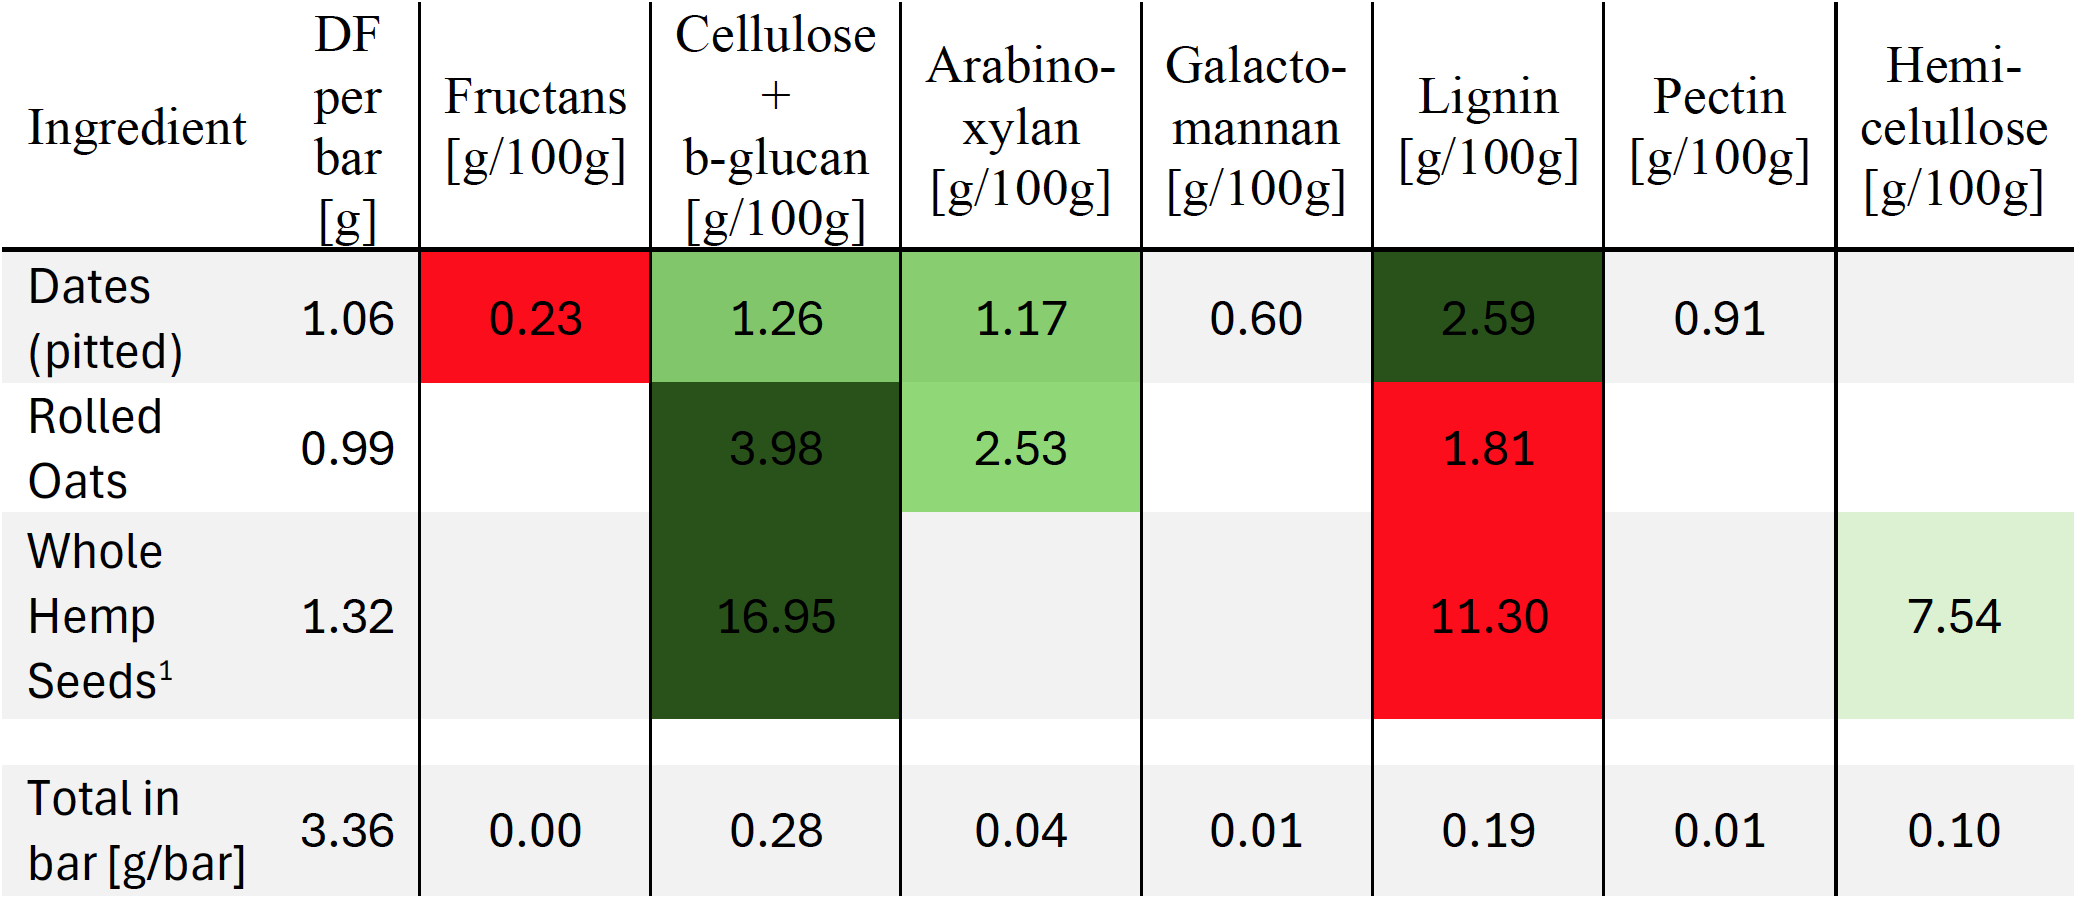
\includegraphics[width=\linewidth]{Figures/tab_df_01.png}
\end{table}

\vspace{1em}
It can be seen in Table 5, that the fatty acid profile is dominated by the polyunsaturated fatty acids (PUFAs). Notably, linoleic acid (LA, C18:2 n-6) and $\alpha$-linoleic acid (ALA, C18:3 n-3) constitutes 69.47\% of the total fatty acids quantified in the bar. These two essential fatty acids, LA (an omega-6) and ALA (an omega-3), cannot be synthetised by the human body and must therefore be obtained through diet. The abundance in the fatty acid profile highlights the nutritional value of the hemp protein bar. Previous studies have reported that LA and ALA from hemp seeds may the nervous system, supporting the health of blood vessels and to protect against cardiovascular diseases \cite*{art_21_hemp_review}. 

\vspace{1em}
Omega-6 tends to have pro-inflammatory pathways, whereas omega-3 supports anti-inflammatory responses. Therefore, maintaining an appropriate balance between these fatty acids is imperative \cite*{art_21_hemp_review}. Although EFSA does not prescribe a fixed omega-6 to omega-3 ratio, its Adequate Intake levels for LA (4\% of energy) and ALA (0.5\% of energy) imply a target ratio of approximately 3\:1. The hemp protein bar provides 1.022 g of omega-6 and 0.430 g of omega-3, yielding a ratio of 2.38\:1, close to, but slightly below the recommended guidelines \cite*{art_22_efsa_fats}. 

\vspace{1em}
As stated, EFSA has set the Adequate Intake levels for LA and ALA to 4E\% and 0.5E\%, respectively. Based on a diet of 2000 kcal, this corresponds to approximately 8.9 g/day of LA and 1.1 g/day of ALA. 



\vspace{1em}
The hemp protein bar will provide roughly 11.5\% and 39\% of the daily requirements of LA and ALA, respectively. Although the substantial contribution to the daily fatty acid intake, these levels does not meet the conditions set by EU for nutrition and health claims. ALA falls below the $geq$ 0.3 g/100kcal threshold for the claim “source of omega-3 fatty acids” \cite*{art_23_regulation1162010}, and LA remains below the $\geq$ 1.5 g/100kcal threshold requires for the claim “contributes to the maintenance of normal blood cholesterol levels” \cite*{art_24_oat_kilning}.

\vspace{1em}
Saturated fatty acids (SFAs) in the hemp protein bar sum to 0.277g per bar, or 13.27\% of the total fatty acid profile. Palmitic acid (C16:0) is the predominant fraction, contributing with 0.199 g per bar. 
Monounsaturated fatty acids (MUFAs) account for 0.360 g of the hemp bar, representing 17.24\% of the 2.09 g total fatty acids. Table 5 illustrates that oleic acid (C18:1, n-9) is the dominant MUFA, consistently ranking among the three most abundant fatty acid fractions in dehulled hemp seeds, whole hemp seeds, and rolled oats. 


\begin{table}[H]
    \centering
    \caption{Contribution of the main dietary fibre sources (dates, rolled oats, and whole hemp seeds) to the hemp seed protein bar,
    expressed as total dietary fibre per bar and distribution of fibre fractions. Coloured cells indicate relative contribution, with light
    green representing lowest top three value and dark green representing the highest of the top three. The red coloured cells indicate the
    lowest value for each ingredient.}
    \label{tab:fatty_acid_tab_01}
    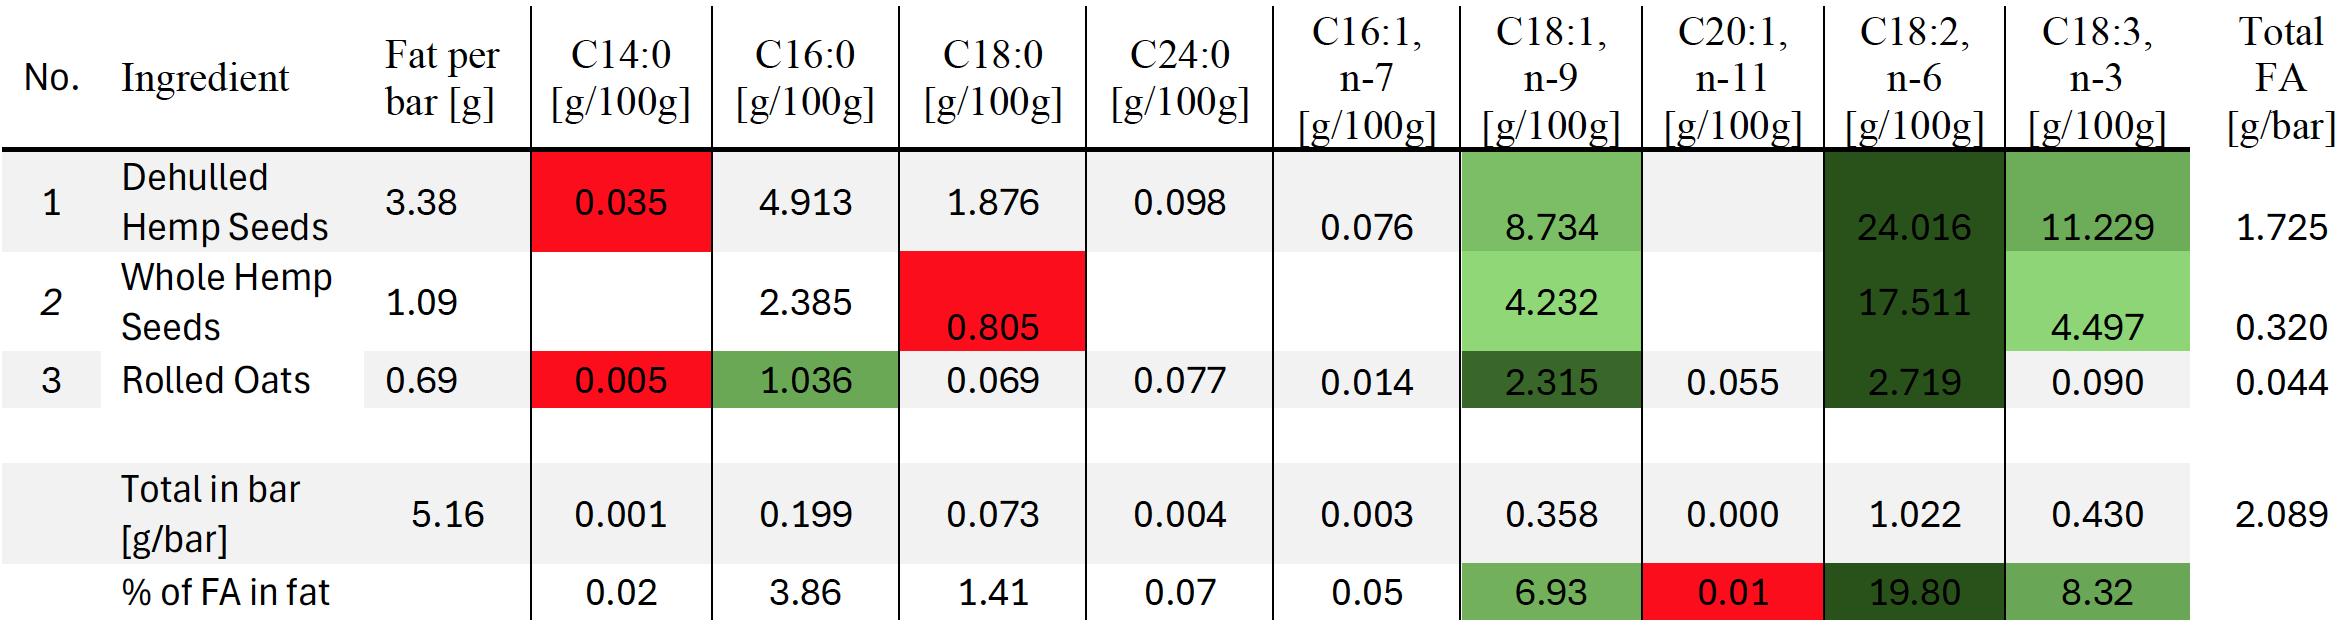
\includegraphics[angle=90,origin=c,width=0.22\textheight]{Figures/tab_fatty_01.png}
\end{table}

\subsection{Comparison with Market Products - ROO'bar}
\subsubsection{Macronutrients Comparison}
A comparison of the macronutrients between the project hemp protein bar and ROO’bar hemp protein bar can be seen in Table 7. The project bar is slightly more energy dense than the ROO’bar, with an energy surplus of 14.7 kcal/100g. The higher energy levels primarily stem from protein and carbohydrates, are present in 9.1 g and 5.3 g greater amounts, respectively. The total fat content is slightly lower in the project hemp protein bar, yet the fat profile appears of a higher quality when reflected by the fraction of fatty acids as the project bar has a surplus of 2.0 g/100g. Although the carbohydrate fraction is higher in in the project hemp bar, the dietary fibre content is lower, indicating that the carbohydrate quality is comparatively less favourable. 

\vspace{1em}
Macronutrient comparison between the ROO'bar hemp protein bar and the project's hemp protein bar, expressed per 100g. The difference column represents (project bar - ROO'bar). Values > 0 are green, indicating a higher content, whereas values < 0 are red, indicating a lower content.

\begin{table}[H]
    \centering
    \caption{Contribution of the main dietary fibre sources (dates, rolled oats, and whole hemp seeds) to the hemp seed protein bar,
    expressed as total dietary fibre per bar and distribution of fibre fractions. Coloured cells indicate relative contribution, with light
    green representing lowest top three value and dark green representing the highest of the top three. The red coloured cells indicate the
    lowest value for each ingredient.}
    \label{tab:fatty_acid_tab_01}
    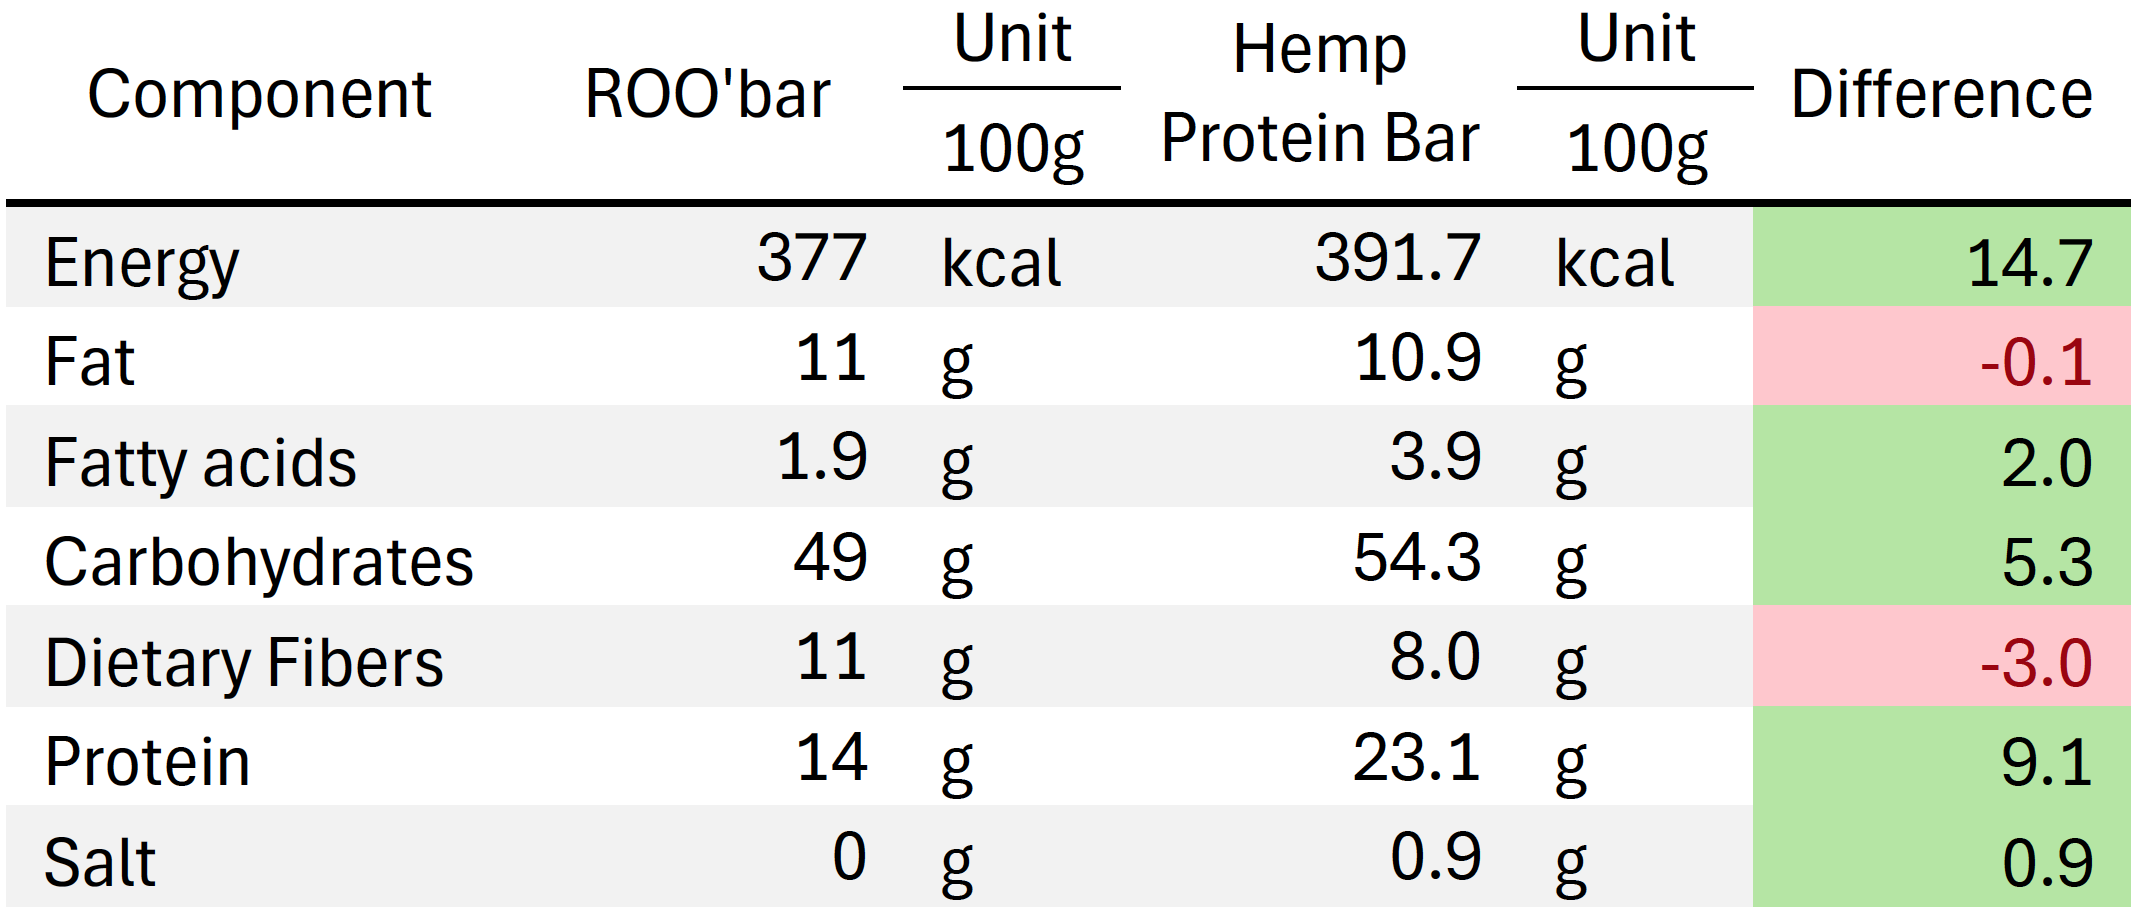
\includegraphics[width=\textwidth]{Figures/tab_comp_comparison_01.png}
\end{table}

\subsubsection{Protein Quality Comparison}
The macronutrient fraction with the largest difference is that of protein. The project hemp protein bar consists of 23.1 g/100g product, compared to the ROO’bar which only consist of 14 g/100g product. This results in a surplus of 9.1 g/100g product in the project bar. This surplus primarily stem from the potato protein isolate in the project bar. In addition, to the potato protein isolate, the project bar also includes dehulled hemp seeds to the formulation, which adds great amounts of high-quality protein. These amounts of protein qualify the project bar for the nutritional claim “high protein” under regulation (EC) No 1924/2006, while the ROO’bar remains just above the threshold for “source of protein”.

\subsubsection{Dietary Fibre Comparison}
The content of dietary fibre in the ROO’bar is greater than that of the project bar. The ROO’bar consist of 11 g/100g dietary fibre, whereas the project bar only consists of 8 g/100g. Both values are above the criteria for the nutritional claim for “high fibre” when expressed in g/100g, although neither of the protein bars reach the required concentration when expressed in g/100kcal. The lower content of fibre in the project bar reflects the dehulling processing step, where the fibre rich hull is removed. In contrast, the ROO’bar formulation relies on hemp protein isolate which is richer in dietary fibres than potato protein isolate. Consequently, while the project bar provides a higher fraction of carbohydrates, the ROO’bar has a comparatively higher quality of carbohydrate profile with respect to dietary fibre. 

\subsubsection{Fatty Acid Profile Comparison}
Although the total fat content in the two bars is nearly identical with the projects hemp protein bar containing 10.9 g/100g and the ROO’bar 11.0 g/100g, the fatty acid profile differs substantially. The fatty acid fraction of the project bar contains 3.9 g/100g, more than twice the amount in the ROO’bar that contains 1.9 g/100g. Table 5 shows that this difference is attributed to the high levels of PUFAs in both whole hemp seeds and dehulled hemp, particularly LA and ALA. The resulting ratio between these fatty acids in the project bar, are approximately 2.4\:1, which is close to the EFSA’s recommended range for balance between omega-3 and omega-6 fatty acids. Neither of the products reach the threshold for authorised EU health claims, but the higher levels of PUFA in the project bar indicates a superior quality lipid profile.

\section{Environmental Impact - sustainability Perspective}
Looking at environmental impacts of the hemp seed bar, it is interesting to investigate the impacts from the hemp seeds, as dehulled and whole hemp seeds contribute to a large proportion of the ingredients (Table XX). As a crop, hemp is considered carbon-negative because it absorbs more carbon from the air during growth than it yields during its production. E.g. one ton of harvested hemp stem absorbs approximately 1.6 tons of CO2, equating to 9–13 tons of CO2 absorption per hectare. (Chapter 1 hemp book \& hemp nutritional value PDF). To compare environmental impacts from different food products life cycle assessment methods are often used. Life cycle assessment methodologies have some limitations due to the methodological choices. It is important to be aware of both what is included and excluded from the assessment e.g. what source of power the calculation is made from. However, International Organization for Standardization (ISO) standard exists for life cycle assessments (Bjørn et al. 2017). Though it is important to be aware that life cycle assessments may fail to provide sufficient guidance on environmental, and nutrition impacts that users should be capturing when comparing the overall sustainability and health impacts of different food products. (McLaren et al. 2021).   

\vspace{1em}
Depending on the genotype and agronomic practices of the hemp seed production, results from a lifecycle assessment revealed that the carbon footprints for most genotypes are below 0.675 kg CO2 eq for 1 kg produced hemp seeds and for the genotype with the lowest carbon footprint it is reported to be 0.161 kg CO2 eq for 1 kg produced hemp seeds. The environmental impacts of hemp seed production were analysed with a focus on the agronomic practices such as changing genotype, plant density, and N fertilization in a Mediterranean environment in central Italy. Though it is noted that the lowest carbon footprint is comparable with other crops, e.g., 0.186 kg CO2 eq for soybeans. (Campiglia et al. 2020).

\vspace{1em}
Moreover, the cultivation of hemp positively affects soil health and water quality, and it supports wildlife by providing habitat and food. (Chapter 1 hemp book) Hemp has deep tap roots that contribute to improved soil structure and carbon storage. (Processering af hamp – industrial hemp pdf) The deep root system also allows for efficient water uptake, contributing to a lower water footprint compared to many other crops. This makes it a more resource-efficient choice for food production. (Processering af hamp – industrial hemp pdf). Furthermore, hemp crops can remediate organic contaminants and heavy metals from the soil, making them suitable for use on land unsuitable for other food crops. Expanding hemp grain production not only supports environmental sustainability in agriculture but can also deliver substantial social benefits, particularly for low-income groups, rural communities, and other socially or economically disadvantaged populations. (Chapter 1 hemp book)

\vspace{1em}
In this report the focus is on a hemp seed bar and not on whole diets, which gives rise to the possibility of overlooking the interplay between the amount of nutrients in the studied food product, and the amount of nutrients from other foods that an individual has eaten. For example, the hemp seed bar may be a main contributor to total vitamin E intake of a person who consumes few other foods that contain vitamin E. In contrast, for a person who consumes many other foods that contain vitamin E, the vitamin E content in the hemp seed bar may only represent a small proportion of their total vitamin E intake. When summarizing a nutritional value of a food product, e.g. based on its nutrient density, the fact that the analyzed food product is part of a whole diet is ignored. To complex it even more the ingestion of sufficient quantities of nutrients is no guarantee of nutrition because the nutrients need to be bioavailable to provide nutrition and bioavailable nutrients starts with bioaccessible nutrients. To really make life cycle assessment studies useful, the nutrient aspect of the food product is an important aspect to consider. It can either be assessed in parallel with the environmental impacts or by using methods that integrate the two dimensions such as nutritional life cycle assessment where reference nutrient intake values are incorporated. (McLaren et al. 2021).

\vspace{1em}
When looking into existing literature, it is found that data lack on nutritional life cycle assessments of hemp seeds, but the existing data on life cycle assessments of hemp seeds suggest that hemp seeds have low carbon footprints and studies of the nutritional value of hemp seeds indicate that hemp seeds are good sources to multiple nutrients that are easily digestible in humans as mentioned previously. (Tănase et al. 2024; Campiglia et al. 2020). 

\vspace{1em}
To calculate the carbon footprint of a food product, a database such as CarbonCloud can be a useful tool (CarbonCloud n.d.). It is a database built on models that follow the ISO 14067, which is the international standard to assess carbon footprint. (McLaren et al. 2021). The carbon footprints in the CarbonCloud database are divided into 5 categories: Agriculture, transport, processing, packaging and storage. Currently, there is no calculations of a hemp seed bar, as presented in this report. But when looking at excising calculations on products such as an energy bar, the biggest contribution to the carbon footprint is agriculture which covers all the inputs from biological processes such as the production and use of fertilizer and pesticides, as well as the energy use for machinery and refinement processes on the farm. As the second largest contribution processing is found and then packaging. Most probably the hemp seed bar would have a similar distribution in a carbon footprint calculation and careful and optimised agriculture practices for all the ingredients are very important to produce a product with a low carbon footprint which make studies such as Campiglia et al. (2020) highly relevant, because many parameters can be adjusted in the agronomic practices.
 
\section{Conclusion}
In conclusion, the hemp seed protein bar developed in this project offers a nutritionally rich and environmentally sustainable snack option. The bar's formulation, which includes dehulled hemp seeds, potato protein isolate, rolled oats, and other wholesome ingredients, results in a balanced macronutrient profile with high protein content, dietary fibre, and healthy fats. The processing methods employed, such as dehulling and light roasting of hemp seeds, enhance the bioavailability of nutrients while reducing antinutritional factors.

\vspace{1em}
The amino acid profile of the bar confirms it as a complete protein source, with all nine essential amino acids present, supporting muscle maintenance and growth. The dietary fibre content, primarily from whole hemp seeds, dates, and rolled oats, contributes to digestive health and overall well-being. The fatty acid profile is dominated by polyunsaturated fatty acids, particularly linoleic and $\alpha$-linolenic acids, which are essential for cardiovascular health.

\vspace{1em}
When compared to existing market products, such as the ROO'bar hemp protein bar, the project bar demonstrates superior protein content and a more favourable fatty acid profile, although it has a slightly lower dietary fibre content. The environmental impact of hemp cultivation further enhances the bar's appeal, as hemp is a carbon-negative crop that supports soil health and biodiversity.

\vspace{1em}
Overall, the hemp seed protein bar represents a promising addition to the market, catering to health-conscious consumers seeking nutritious and sustainable food options. Future research could focus on further optimizing the formulation for taste and texture, as well as conducting comprehensive life cycle assessments to quantify the environmental benefits of hemp-based products.


%\chapter{Product Concept}
\setlength{\headheight}{22.94003pt}
\addtolength{\topmargin}{-10.22661pt}

It is estimated that only 35\% of the globally produced plant protein is consumed by humans. Meanwhile the current market offers a wide range of plant-based proteins available which are well fitted for human consumption. Common choices include formulations with oat, wheat, hemp, soy and pea to name a few (Gorissen et al., 2018). The Cannabis sativa L., a Cannabaceae known as ‘‘hemp’’ is of increasing interest because it is highlighted as an environmentally friendly and economically high-potential crop. Its history as a source for medicine, fiber and food dates back 6000 years, and the cultivation of hemp with close to no levels of tetrahydrocannabinol (THC), the psychoactive compound found in cannabis, has increased to use in foods since strains with a THC content below 0.3\% was approved in EU in 1996. Among its many advantages are fast growth and low dependency on pesticides, which benefits biodiversity and healthy soils. Furthermore, its seeds provide a valuable source of nutrients. (Chapter 6 Industrial Hemp Seed). Globally, the trend of increasing interest for hemp seeds is clear, as the production increased from 2,718 tons to 5,449 tons between 2015 and 2020. 

\vspace{1em}
Thus, developing a convenient hemp-based bar would harness the many benefits of the not-so-novel ingredient that is hemp seed. Below is a mock up of the Hemp Protein Bar (figure 4).

\begin{figure}[H]
    \centering
    \includegraphics[width=0.54\linewidth]{Figures/fig_prod_concept_01.png}
    \caption{AI-generated illustration of a medieval marketplace. Generated using DALL·E 3 (OpenAI, 2025) with the prompt: "Mock up of a hemp bar picture half coved in chocolate ".}
    \label{fig:prod_concept_01}
\end{figure}


\section{Macronutrients in Hemp Seeds}
Hemp seeds typically contain around 20-30\% protein, 25\%-35\% lipids, 20-30\% carbohydrates and 4-7\% of ash (Figure 5). It has a balanced composition with particularly low starch content. (Montero et al 2023) 

\begin{figure}[H]
    \centering
    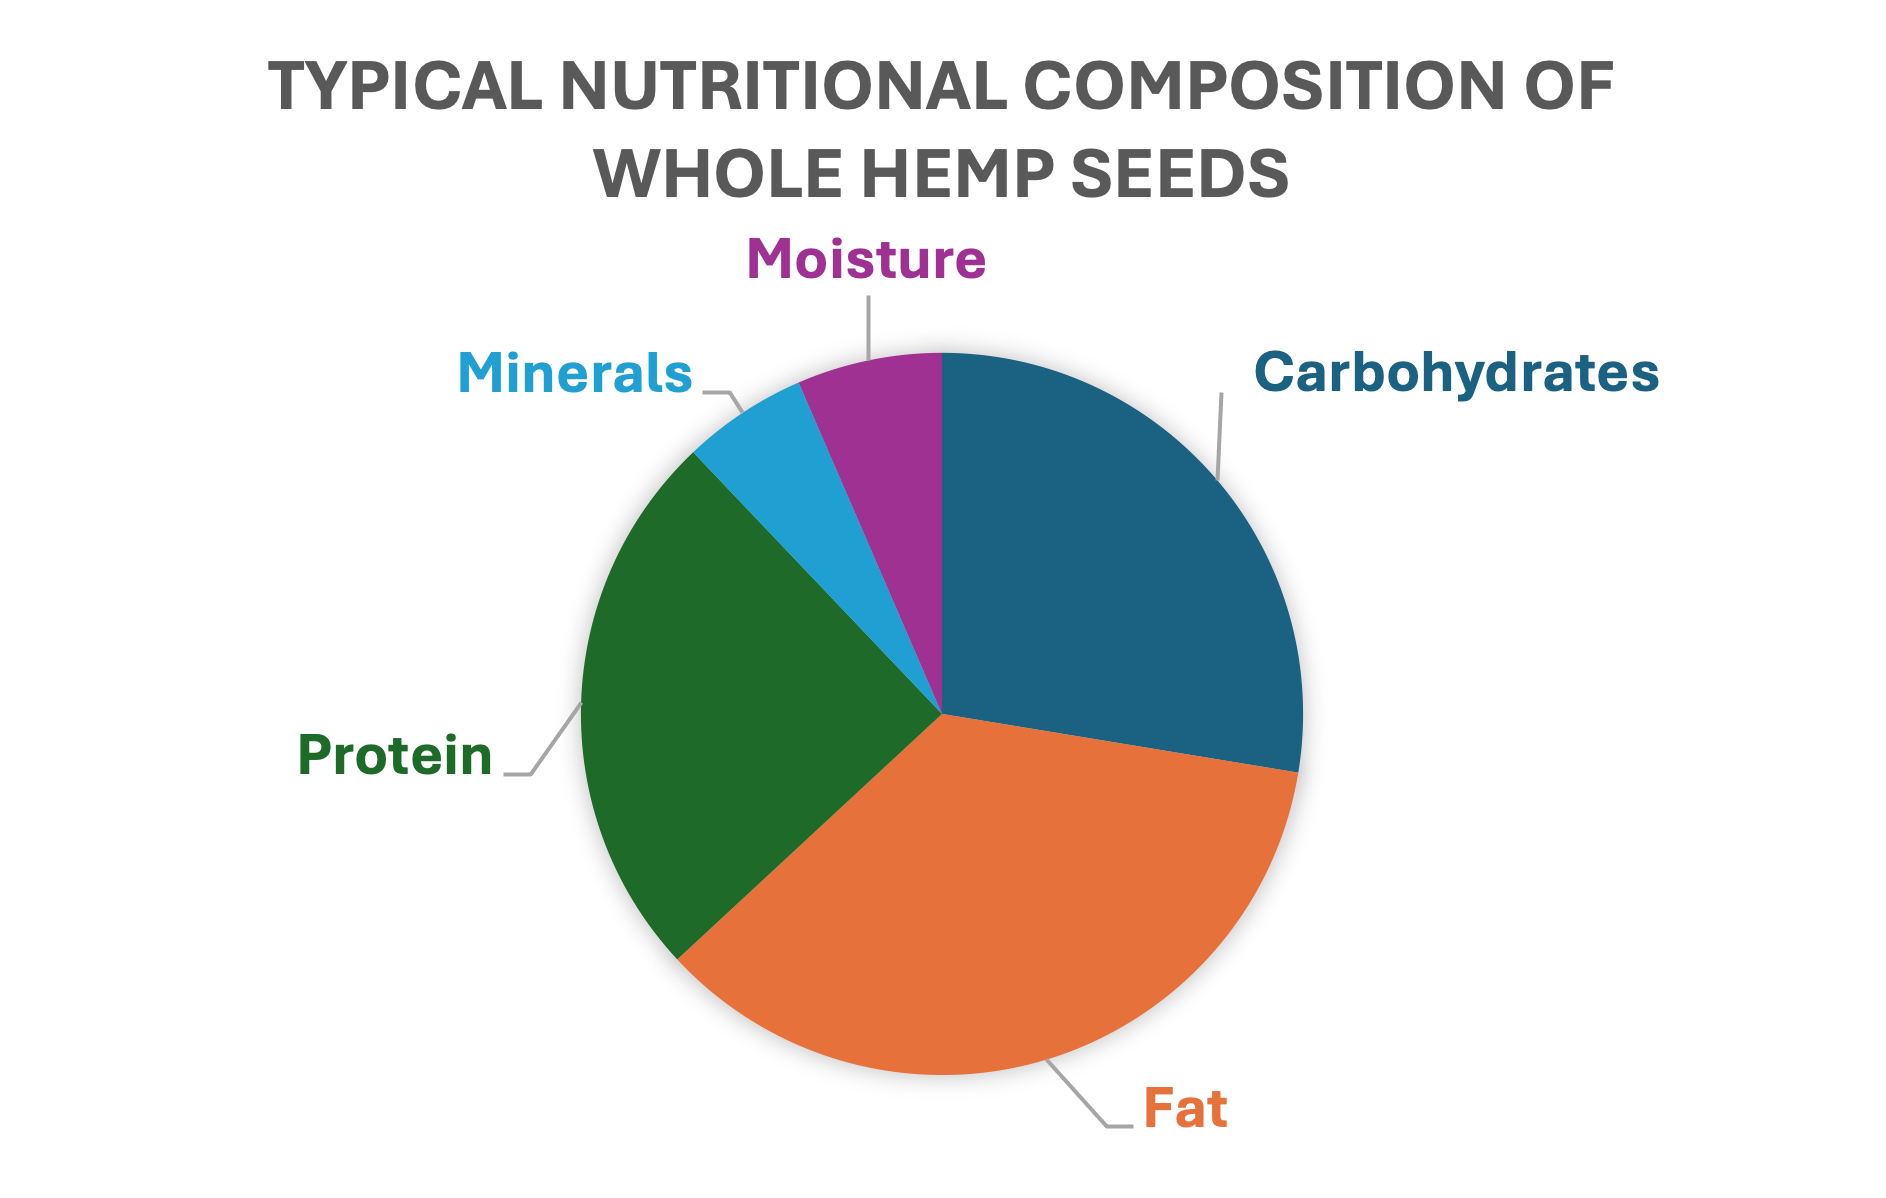
\includegraphics[width=0.75\linewidth]{Figures/fig_prod_concept_02.png}
    \caption{Composition diagram of whole hemp seeds}
    \label{fig:prod_concept_02}
\end{figure}

\subsection{Protein}
Hemp seeds are an excellent source of high-quality protein, typically containing 20–30\% protein, with dehulled hemp seeds having even higher protein contents, ranging from 30\% to 38\%. (chapter 4 hemp seed book). The two main proteins in hemp seeds are albumin (33\%) and edistin (65\%), which have very similar structures to plasma proteins which helps the digestibility in humans. Hemp seeds provide a complete amino acid profile, containing all nine essential amino acids required by humans, making them comparable to other high-quality proteins like egg white and soybeans (Chapter 10). 

\vspace{1em}
The protein is also particularly rich in arginine, glutamic acid, and aspartic acid, where arginine is especially valuable as it is a precursor to nitric oxide, which enhances blood flow and helps maintain normal blood pressure, contributing to cardiovascular health (chapter 11 hemp book)
Hemp proteins are highly digestible, with dehulled hemp seeds demonstrating superior protein digestibility (83.5–92.1\%) (hemp nutritional value). This is partly attributed to the absence of protease inhibitors in hemp seeds (Hemp seed bioactivity). 

\vspace{1em}
A study has analysed the macronutrient composition and protein quality of 30 hemp seed products from Western Canada, including whole seeds, dehulled seeds, and hemp seed meal. Crude protein, fat, and amino acid profiles were determined, and protein quality was assessed using the Protein Digestibility-Corrected Amino Acid Score (PDCAAS) method, based on a rat bioassay and FAO/WHO amino acid requirements for young children. Average protein content ranged from 24.0\% in whole seeds to 40.7\% in hemp seed meal. Protein digestibility was 84–98\%, with protein digestibility-corrected amino acid score (PDCAAS) values of 46–66\%, highest in dehulled seeds. The protein digestibility-corrected amino acid score of dehulled hemp seed is comparable to lentils and is about half that of casein, and almost twice that of almonds (chapter 10 hemp seed book)

\subsection{Fatty Acids}
Hemp seed oil is primarily composed of polyunsaturated fatty acids, PUFA (over 80\%) including fatty acids like essential linoleic acid (omega-6) and alpha-linolenic acid (omega-3). (Chapter 10 hemp seed book) Dehulled hempseeds have a healthy balance of omega-6 to omega-3 polyunsaturated fatty acids (2.5:1) (Chapter 1 hemp book)

\vspace{1em}
Unsaturated fatty acids help protect against cardiovascular disease, obesity, diabetes, and inflammation. EFSA recommends an optimal omega-6/omega-3 ratio of 3:1 to 5:1. Hemp seed oil typically shows a ratio of 2.5–3.5:1, which is a desirable range linked to lower chronic disease risk. (Hemp nutritional value pdf)

\section{Carbohydrates}
About 98\% of the carbohydrates in hemp seeds are dietary fiber, mainly insoluble dietary fibers (80\%), such as cellulose, lignin and hemicellulose. Dietary fiber resists enzymatic digestion in the small intestine and undergoes partial or complete fermentation in the large intestine. The remainder of the carbohydrates in hemp seeds is starch. Therefore, hemp seeds are considered a low-starch food and an excellent source of dietary fiber. (Hemp nutritional value pdf) 

\vspace{1em}
The dietary fibers from hemp seeds are associated with positive effects on the digestive tract support by acting as prebiotics. The fermentation of fibers in the colon generates short-chain fatty acids that have beneficial roles in the body. (Hemp seed bioactivity pdf). In the Western countries the consumption of dietary fiber is lower than the recommended intake, making hemp seeds an attractive ingredient to meet the recommended daily intake of dietary. However, processing might affect the amounts of dietary fibers in hemp seeds. 

\section{Micronutrients: Vitamins and Minerals}
Hemp seeds are rich in vitamins and minerals. Just 50 mg of hemp seed can supply at least half of the recommended daily allowance of copper, magnesium, and zinc, and exceed the recommended daily allowance of the vitamins A, D, and E. (Chapter 1 hemp book) Hemp seeds also contain other micronutrients such as phosphorus, potassium, calcium, sodium, iron, and manganese. (Chapter 4 hemp book). Hemp seed oil contains fat-soluble vitamins, in particular vitamin E (tocopherols) and vitamin A which respectively has an antioxidant role and is beneficial for skin integrity and Vitamin D is important for bone health and the immune system (Hemp nutritional value pdf)

\vspace{1em}
Besides the macro- and micronutrients, secondary metabolites, such as terpenes, phytosterols and flavonoids, constitute essential components of the defence response of the hemp plant to biotic and abiotic stresses. However, the composition of these secondary metabolites can be influenced by cultivation conditions, providing a distinct fingerprint of different production regions. It is suggested that these compounds contribute with antioxidative, antimicrobial, and anti-inflammatory properties in the human body. Phytosterols for instance, are not synthesized in humans, but can when ingested from plants, reduce cholesterol levels in the human body by changing the cholesterol solubility in the intestine. (Tănase et al. 2024).

\section{Potential Side Streams}
The industrial hemp plant has a versatile plant body which consists of seeds, leaves, stem, and flowers with several application opportunities depending on the part of the plant. Particularly the stem is a valuable source to produce hemp fiber which can be used for rope, building materials, paper, or textiles. The seeds, dehulled or whole, can be utilized as a food source. The hemp flower can be used to produce cosmetic and pharmaceutical products, including essential oils. When looking further into hemp as a natural source to bast fiber a life cycle assessment reveals that hemp performs better than glass fiber by weight and compared to cotton, hemp requires less water and pesticides to grow although hemp fiber is known to be coarser and stiffer than cotton which has a softer appearance. (Kaur \& Kander 2023). 

\vspace{1em}
When processing the stem to hemp fiber a by-product of shives is made. It can be used to produce hemp concrete which is a bio-composite and carbon-negative alternative to concrete for construction and insulation. (Yano \& Fu 2023). These useful side streams make hemp even more attractive to use as an ingredient in foods. 

\section{Dietary Pattern of the Chosen Consumer Group and Product Fit}
Our hemp seed bar is uniquely positioned to seamlessly integrate into several contemporary dietary patterns, directly addressing the needs and preferences of our diverse target consumer groups within the Millennial and Generation Z age group.

\vspace{1em}
For vegetarians and vegans dehulled hemp seeds are an excellent source of high-quality, plant-based protein. The seeds naturally contain all nine essential amino acids required by humans, offering a complete protein profile that can be challenging to obtain from other plant sources. (Chapter 1 hemp seed book) The protein in dehulled hemp seeds also boasts superior digestibility (83.5\%-92.1\%) compared to whole hemp seeds and hemp meal, making its nutrients more accessible. They also provide a healthy balance of omega-6 to omega-3 polyunsaturated fatty acids (typically 2.5:1 to 3.5:1), which is desirable for overall human nutrition. (Hemp nutritional value pdf) Hemp protein and flour can serve as an alternative for soy ingredients (Chemical composition and biological activities of PDF) 

\vspace{1em}
A health-conscious person or athlete would also use it for its excellent source of protein, especially because of the high value protein composition with the nine essential amino acids. Furthermore, it scores high in terms of digestibility which makes our bar effective for muscle recovery and satiety. (Chapter 10 hemp book) Many athletes need to have control on their calorie needs. Our bar could therefore be an easy boost of calories or be used as a substitute for a snack or meal.
\vspace{0.5em}
The bar is rich in healthy fats, including the beneficial omega-6 to omega-3 ratio, which is important for cardiovascular health and may help prevent chronic diseases. (Hemp nutritional value pdf)

\vspace{1em}
Our bar is also a good source of essential minerals like copper, magnesium, and zinc, and provide vitamins A, D, and E, which also talks to the health-conscious person (Chapter 1 hemp book)

\vspace{1em}
For individuals with dietary restrictions and/or allergies our bar is also a great option, as our bar is naturally gluten-free, making it a safe nutritious option for people with celiac disease or gluten sensitivities. (Chapter 1 hemp book) Hemp proteins are generally considered to have low allergenicity compared to common proteins like soy, dairy, or wheat, broadening its appeal for those with various food allergies. (Chapter 11 hemp book \& Hemp nutritional value pdf)

\vspace{1em}
For environmentally aware consumers our hemp-based product directly supports environmental sustainability due to it having a low environmental impact, actively contributing to improved soil health, water quality, have carbon-negative crops and requiring no or little pesticide use. (Chapter 1 hemp book \& hemp nutritional value PDF \& hemp seed bioactivity) 

\vspace{1em}
The pre-packaged protein bar format offers convenience and time efficiency, requiring no preparation or cleanup for the people on-the-go. It delivers the balanced nutrition derived from dehulled hemp seeds in an easily consumable form, perfectly fitting the needs of busy individuals seeking healthy and convenient dietary options.



%\chapter{Formulation and Raw Materials}
\setlength{\headheight}{12.71342pt}
\addtolength{\topmargin}{-0.71342pt}

The formulation of the hemp seed bar is an important factor, as it regulates the final nutritional composition and determines the parameters for the upstream and downstream processing steps. Using consistent suppliers and high-quality raw materials are key factors in maintaining a predictable, consistent production. Production as such would decrease faults, which reduces waste and ensures safe a safe high-end product to the final consumer. 

\vspace{1em}
Given the lack of sweetness of hemp seeds, the bar is formulated with naturally sweet components such as dried dates and agave sirup. Along with a caramelly flavor, important cohesiveness of the bar is achieved. The dates are dried which reduces water content and thus increases sugar concentration and intensifies flavor. Minimum processing other than dehydration and pitting ensures valuable components such as micronutrients and fibers are included.

\vspace{1em}
To complement the protein value (which lacks in lysine), potato protein isolate is used. During its production, it undergoes heavy processing which concentrates the protein content while reducing other macronutrients, minerals and vitamins (Wagley et al., 2019).

\vspace{1em}
Rolled oats are used as a structural component. It is chosen as it is a gluten free, cheap, readily available raw material known to consumers. It undergoes dehulling, rolling and steaming, which maintains the high fiber content while inactivating lipase enzymes to prevent oxidation and extend shelf life (Ekelund et al., 2024). Ground flax seeds are also included to account for the loss of dietary fibers in Hemp. The flax seeds are grounded to inhibit toxic effects of cyanogenic glycosides (Nowak et al., 2023).

\vspace{1em}
Preprocessing of hemp seeds aims to partially remove the hull/husk (figure 6). The macronutrient profile of the seed is significantly affected by the processing method. Although the formulation does not involve hemp protein isolate, HPI, many studies on this subject point at the effects of preprocessing. 

\vspace{1em}
For example, a study by House et al., 2010 evaluated HPI derived from whole seeds, hemp seed meal, and solely hulls. The study could show that the amino acid composition is different among the three processed raw materials. In the works by Shen et al., 2020 the HPI of dehulled and whole seeds were comprehensively investigated in terms of aromatic components, colour, and protein characterization. Dehulled seeds would increase the extraction yield by 21.52 \% and protein recovery yield (46.90\%) of the HPI. Naturally, the HPI with whole seeds would contain increased amounts of lipids and carbohydrates. The preprocessing also had a profound impact on colour, were whole seeds generated a darker coloured HPI. This matter is further explained in the section “4.1 Effects on Processing”

\vspace{1em}
Vanilla extract, cocoa and sea salt are used to characterize the aroma of the bar. Potentially masking some of the earthy off-flavours from the other ingredients. 


\begin{figure}[h]
    \centering
    \begin{subfigure}{0.45\textwidth}
        \centering
        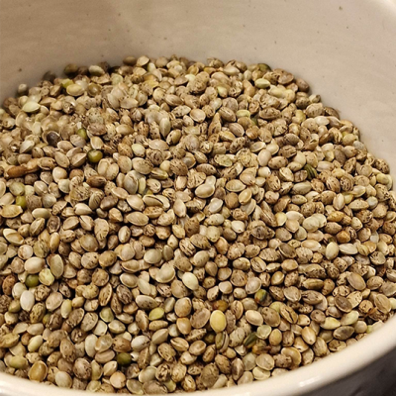
\includegraphics[width=\linewidth]{Figures/fig_formulation_06.png}
        \caption{Whole hemp seeds}
        \label{fig:whole_hemp}
    \end{subfigure}
    \hfill
    \begin{subfigure}{0.45\textwidth}
        \centering
        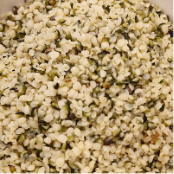
\includegraphics[width=\linewidth]{Figures/fig_formulation_06.1.png}
        \caption{Dehulled hemp seeds}
        \label{fig:dehulled_hemp}
    \end{subfigure}
    \caption{Whole and dehulled hemp seeds (Svensk Hampaindustri, 2025).}
    \label{fig:whole_dehulled}
\end{figure}


%\chapter{Processing and Manufacturing}
\setlength{\headheight}{12.71342pt}
\addtolength{\topmargin}{-0.71342pt}

The production process of the protein bar can be seen on Figure 7.
\begin{figure}[H]
    \centering
    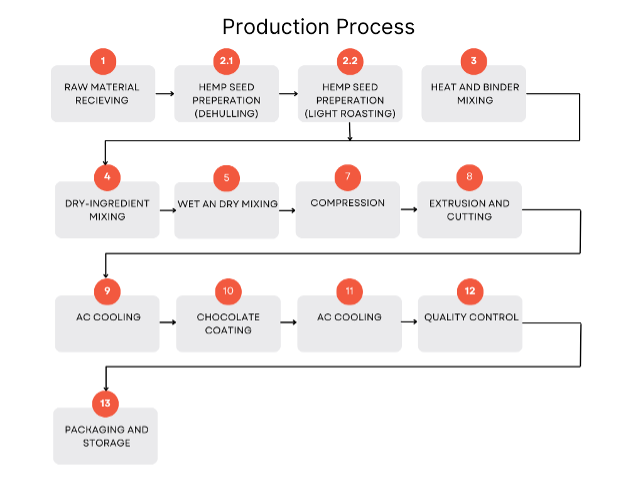
\includegraphics[width=0.8\textwidth]{Figures/fig_process_01.png}
    \caption{A flowchart with a visualization of the production process of the hemp protein bar}
    \label{fig:process_flow_diagram}
\end{figure}

\textit{Sourcing and preparing} raw materials – all ingredients are inspected for quality and stored under appropriate conditions to maintain freshness. All ingredients are weighed and portioned accurately according to the recipe formulation, ensuring batch-to-batch uniformity. This ensures that only safe, high-quality, and properly measured ingredients enter the mixing stage, laying the foundation for a consistent protein bar in terms of flavor, texture, and nutritional profile.

\vspace{1em}
\textit{Dehulling hemp seed} – Increases absorption of proteins and nutrients.

\vspace{1em}
\textit{Light roasting} – of the dehulled hemp seed (75°C-80°C) - improves digestibility, and reduces anti-nutritional factors and lower microbial load.

\vspace{1em}
\textit{Mixing} to homogeneous mixture – evenly distributed throughout the mixture providing a consistent texture and flavor in every bar. Time and temperature in mixing are controlled to ensure that every batch is consistent.

\vspace{1em}
\textit{Compression} – shaping the mixture into a form that is suitable for further processing. Using large presses ensures a uniform sheet, which helps create consistency in texture and flavor throughout the bar.

\vspace{1em}
Extrusion and cutting – A combination of extrusion and cutting technologies are used to shape the mixtures into bars. The extrusion process forces the mixture through a die, after which a knife cuts the long bars into the desired length.

\vspace{1em}
AC cooling – is used to ensure that the bar maintains the desired temperature throughout the process, as mixing and pressure from extrusion can increase the temperature of the product.

\vspace{1em}
Chocolate coating – for flavour.

\vspace{1em}
\textit{AC cooling} – to solidify the chocolate.

\vspace{1em}
\textit{Quality control} – Both automated sensors and visual inspection for defects or foreign objects. Taking samples to ensure that our product meets quality standards, as well as for example checking that the product contains enough protein to be claimed as a product with a high protein content. 

\vspace{1em}
\textit{Packaging} – wrap each bar individually and in a material that keeps the protein bar safe and to ensure that the bar does not undergo oxygenation and to preserve freshness. This process also includes labelling and coding to ensure traceability and compliance with regulatory requirements.

\section{Effects on Processing}
Hemp seeds contain several antinutritional, such as phytic acid, tannins and saponins. The presence of tannins and saponins can reduce the bioavailability of nutrients and disrupt both metabolism and digestive functions (kapitel 4 hampbog). The presence of phytic acid can lead to mineral deficiencies (e.g. iron, zinc and calcium), as it can inhibit the absorption of these. (kapitel 10 hampbog). Polyphenols, of which tannins are a part, are often found in the shell of hemp seeds (hemp nutritional value pdf). The same applies to phytic acid. Studies have shown that there is significantly more phytic acid present in whole hemp seeds 3.5 g/100g compared to 2.1 g/100g in hulled hemp seeds. That is a reduction of 40\%. (kapitel 4 hampbog).

\vspace{1em}
According to House et al. (2010), whole hemp seeds have a protein digestibility of approximately 84–86\% and a protein digestibility-corrected amino acid score (PDCAAS) value of 49–53\%, while dehulled hemp seeds reach a digestibility of 91–97\% and a PDCAAS value of 63–66\%. This improvement is primarily due to the fact that the hull contains a large part of the fiber fraction of the seed, which inhibits digestibility, so when the hull is removed, the fiber content is significantly reduced, making the protein more available and thus improving the overall protein assessment (PDCAAS) (Evaluating the Quality of Protein from Hemp Seed pdf.) Therefore, by using a majority of dehulled hemp seeds instead of whole hemp seeds, we reduce the content of antinutrients and increase the nutritional quality of the protein.

\vspace{1em}
Plant proteins naturally contain antinutritional factors such as trypsin inhibitors, glucosinolates, phenols and phytates, together with a high content of dietary fiber, which can negatively affect protein and amino acid digestibility and bioavailability. Heat processing can effectively help to remove or reduce these compounds, leading to higher protein digestibility. However, high heat treatment can have negative effects as it can affect the chemical transformations of amino acids. Some amino acids, such as lysine, can be chemically transformed and become unavailable during heat treatment or other severe processes, leading to problems such as the formation of Maillard reaction products. This underlines the need for appropriate processing conditions to avoid such. (Protein Quality Report No 92 web version .pdf)



\begin{table}[h]
    \centering
    \caption{Protein digestibility-corrected amino acid scores of hemp protein sources in comparison to other food proteins. (Evaluating the Quality of Protein from Hemp Seed pdf.)}
    \label{tab:process_table_01}
    \begin{tabular}{l c}
    \hline
    \textbf{Protein source} & \textbf{PDCAAS (\%)} \\
    \hline
    Casein               & 100 \\
    Egg white            & 100 \\
    Beef                 & 92  \\
    Soy protein isolate  & 92  \\
    Chickpeas (canned)   & 71  \\
    Pea flour            & 69  \\
    Kidney beans (canned)& 68  \\
    Dehulled hemp seed   & 61  \\
    Pinto beans (canned) & 57  \\
    Rolled oats          & 57  \\
    Lentils (canned)     & 52  \\
    Hemp seed            & 51  \\
    Hemp seed meal       & 48  \\
    Whole wheat          & 40  \\
    Almond               & 23  \\
    \hline
    \end{tabular}
\end{table}

\vspace{1em}
At the same time, a study has shown that hemp protein isolates improved proteolysis when heated at 75 °C and 80 °C, but already at 90 °C it caused reduced proteolysis. (hemp seed bioactivity pdf) Therefore, we have chosen to lightly roast our dehulled hemp seeds to achieve the highest possible protein absorption, but with an eye not to reach too high a temperature, as we want to avoid a greater loss of lysine and reduced proteolysis.
%%\chapter{Final Nutritional Profile of the Bar - Lucas}
\setlength{\headheight}{12.71342pt}
\addtolength{\topmargin}{-0.71342pt}

\section{Final Nutritional Profile of the Bar - Lucas}
\subsection{Nutritional Composition Overview}
In this section of the report, the macronutrient composition of the hemp seed protein bar is examined, namely protein, dietary fibre, and fatty acids. The final nutritional profile was estimated based on the formulation and calculated contributions of each ingredient. Table 6 shows the magnitude of each ingredient in the bar, where the highlighted cells represent the top contributors that will be examined in greater detail. This section further outlines the amino acid and fatty acid spectrum, evaluates potential nutrition and health claims considering EU regulations and EFSA opinions, and compares the bar’s profile to existing market products.


    \begin{table}[t]
        \caption{The table indicates the 10 ingredients that the product is made of, and the respective values for three of the most notable macronutrients and moisture content. The top five contributor for each of the factors is highlighted in green, ranging from dark to light-green from highest to lowest value corresponding to the amount of the macronutrient in the bar. }
    \label{tab:df_amino_acids_01}
    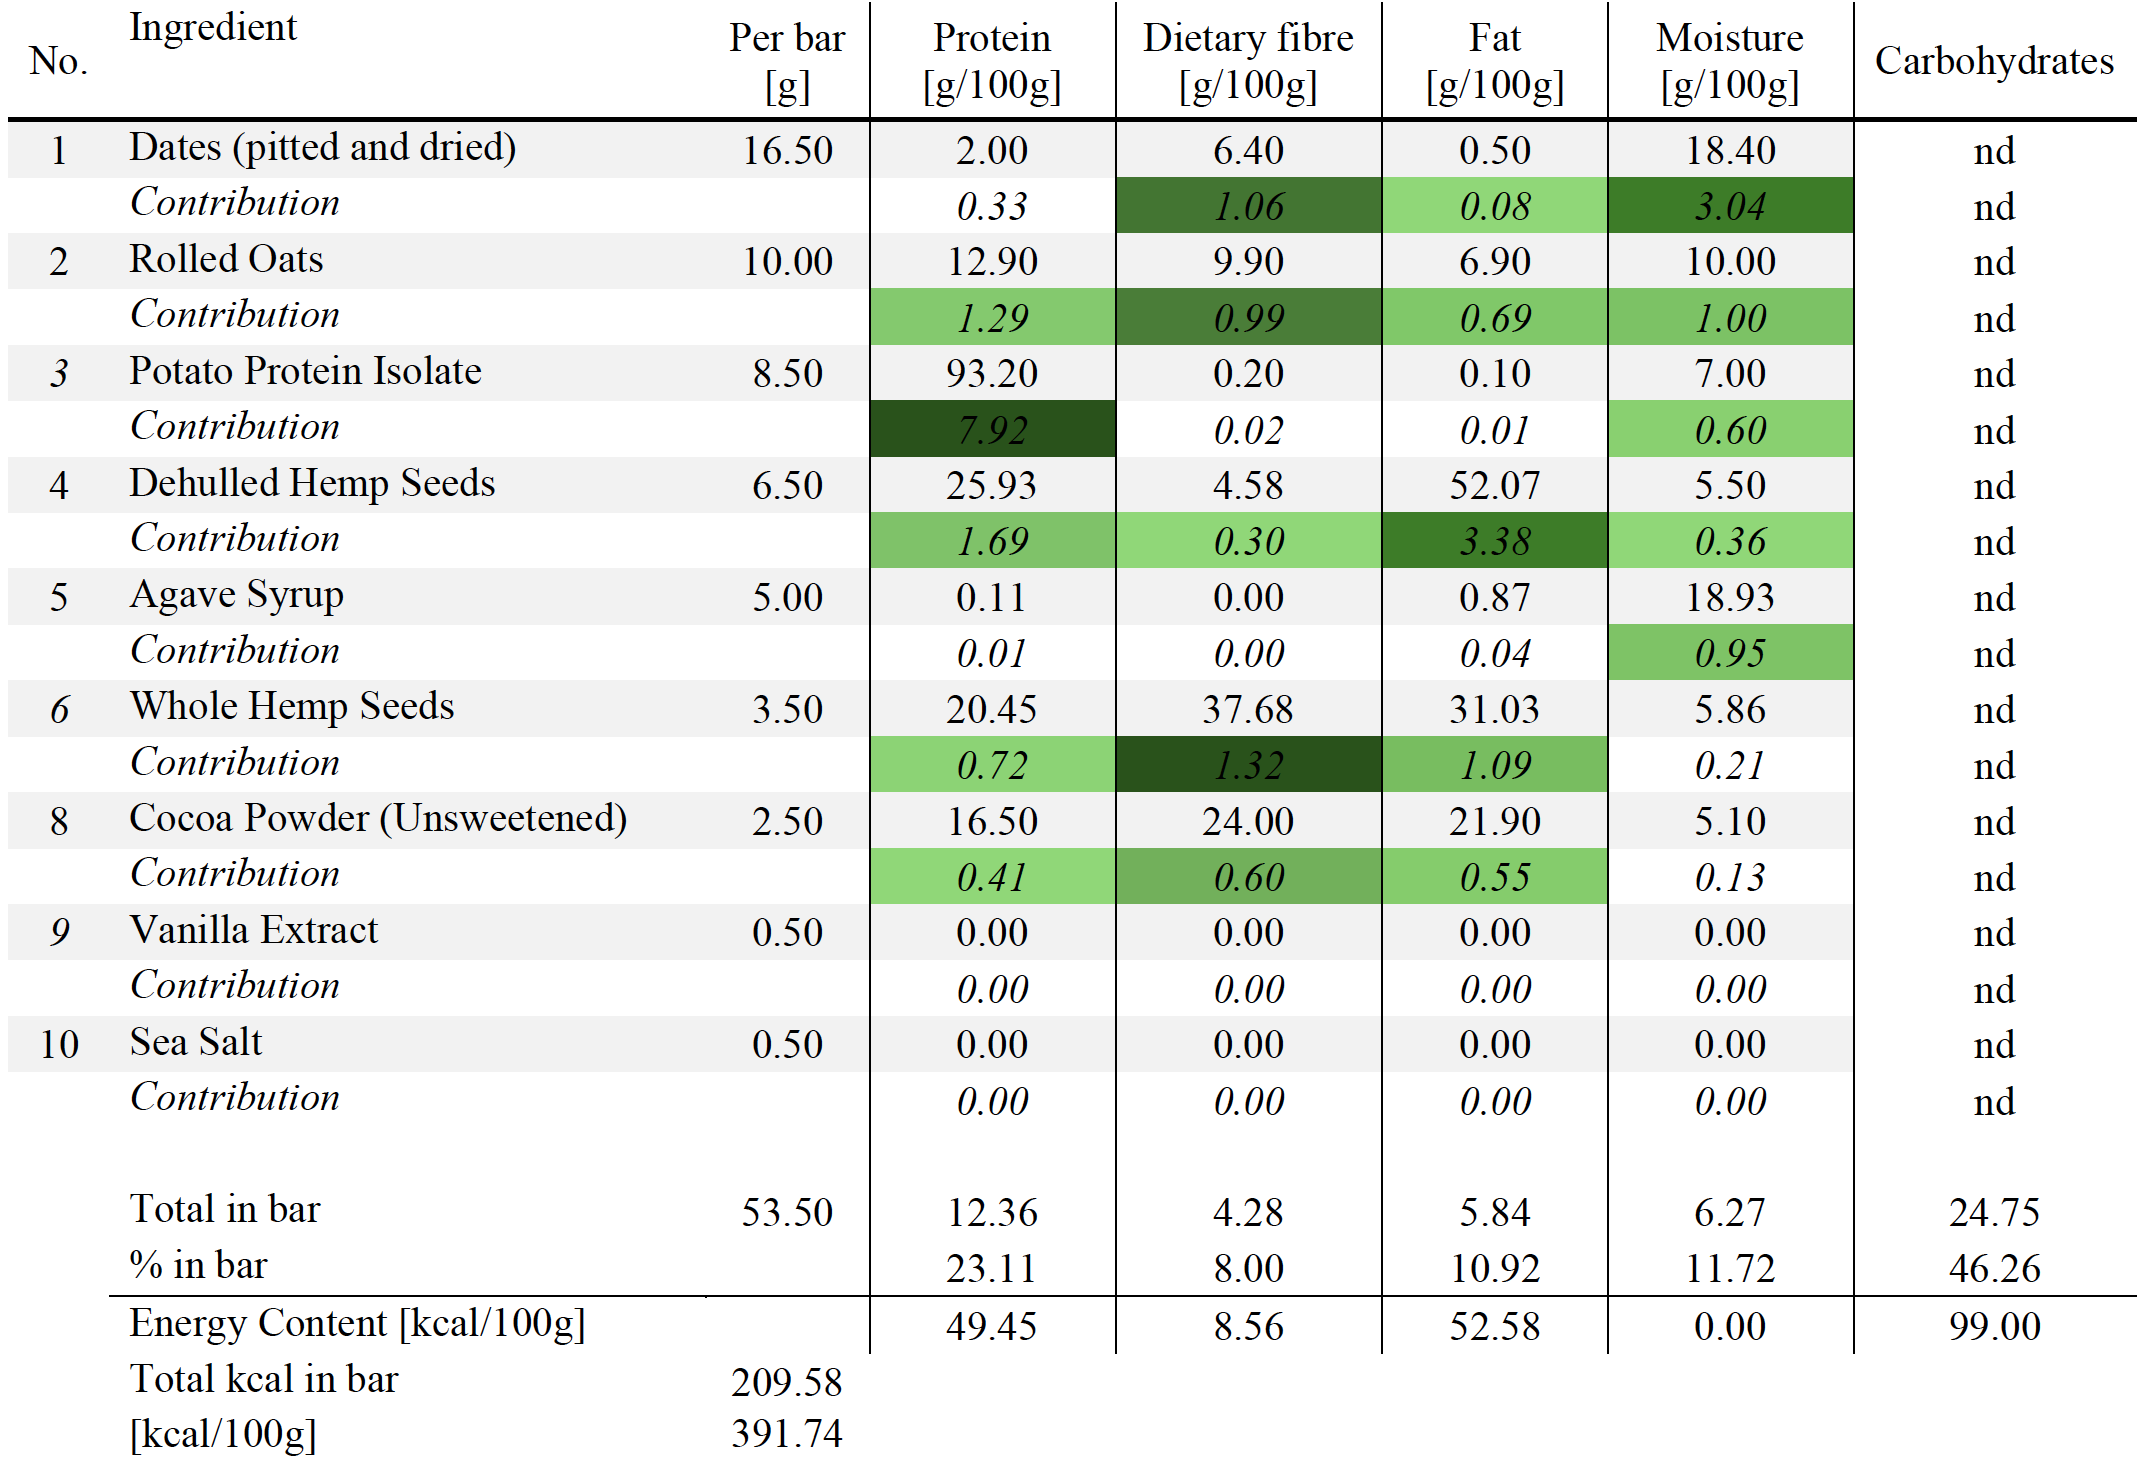
\includegraphics[width=\linewidth]{Figures/tab_overall_ingredients_01.png}
\end{table}

\subsection{Macronutrient Composition}
As shown in Table 6, the hemp seed protein bar delivers 209.6 kcal per 53.5 g bar, with a macronutrient profile characterised by 12.36 g protein, 4.28 g dietary fibre, 5.84 g fat, 6.27 g moisture, and 24.75 g carbohydrates. This balance between protein, fibre, and healthy fats underlines the bar’s potential as a nutrient-dense snack.

\vspace{1em}
The overall macronutrient profile was calculated using data from various sources to determine the contribution of each ingredient. For each raw material, published nutrient values were combined with the amount used per bar (g) to estimate the contribution of the respective ingredient. The calculations followed Equation 5.1. 


\begin{equation}
    \text{Contribution [g]} = 
    \frac{\text{Nutrient content [g/100g]} \times \text{Ingredient weight [g]}}{100}
    \label{eq:contribution}
\end{equation}

This approach was applied for protein, dietary fibre, fat and moisture. Carbohydrates were excluded from direct analysis, thus their content was derived by calculating the difference, as outlined in Equation 5.2. 

\begin{equation}
    \text{Carbohydrates [g]} = 
    \text{Total weight [g]} - (\text{Protein} + \text{Fat} + \text{Dietary fibre} + \text{Moisture})
    \label{eq:carbohydrates}
\end{equation}

The energy content of the bar was subsequently estimated while adhering to the conversions factors defined in regulation (EU) no. 1169/2011 (protein 4 kcal/g, carbohydrates 4 kcal/g, fibre 2 kcal/g) art\_17. The energy content for moisture was assumed to contribute with 0 kcal/g, thus neglected in the calculations. 

\vspace{1em}
Based on published nutrient values and the calculations described, the bar (53.5 g) provides 209.6 kcal, equivalent to 391.7 kcal/100 g. Its macronutrient composition - 23.1\% protein, 8.0\% dietary fibre, and 10.9\% fat - qualifies the product for the nutrition claims, “High protein” and “High fibre.” These claims comply with the conditions defined in the Annex of Regulation (EC) No 1924/2006, which governs nutrition and health claims across the European Union art\_16.    

\subsubsection{Protein Content and Quality}
Protein intake is essential for muscle protein synthesis, but the source and type of protein substantially influences its digestibility and utilisation. Since humans cannot synthesise essential amino acids, these must be obtained through diet. Consequently, the overall protein composition, and particularly the essential amino acids profile, is a key to determine protein quality art\_08.

\vspace{1em}
The hemp seed protein bar provides a total of 12.36 g protein per bar. As shown in Table 6, the main contributors for protein are potato protein isolate, rolled oats and dehulled hemp seeds. Dehulling is a processing step which has a significant effect on protein quality. It improves digestibility and reduces antinutritional factors, while also elevating the protein fraction of the hemp seed (hemp\_book). To further characterise the protein profile, Table 3 presents an in-depth analysis of the protein composition, with respect to each ingredient’s amino acid composition. The data was compiled from multiple sources, yet the methodologies used for amino acid determination has been similar across the studies (FridaFood, art\_08, art\_09, art\_10).

\vspace{1em}
The amino acid profile derived from the three main protein contributors includes all nine essential amino acids, confirming the bar as a complete protein source for the consumer. In each of the three main protein contributors, Leucine is the most abundant essential amino acid. Overall, Leucine makes up 5.32\% of the total amino acids contributed by the three ingredients. The combined amount of essential amino acids, derived from these contributors, amounts to 2568.83mg, of which Leucine alone constitutes 22.54\%.

\vspace{1em}
For both rolled oats, and dehulled hemps seeds, the lowest contribution stems from Tryptophan. General consensus, regarding the hemp seed amino acid profile identifies Lysine as the limiting essential amino acid. However, published values vary considerably depending on the analytical methods used, cultivation conditions and cultivar (hemp\_book). 

\vspace{1em}
Conversely, Tryptophan was not identified in published data for potato protein isolate, suggesting a scarce amounts present. For this ingredient, Methionine and Histidine was reported as the limiting essential amino acids, only contributing with 1300 mg/100g, which is substantially lower than the levels of the other essential amino acids. 

\vspace{1em}
The hemp seed protein bar exhibits an overall balanced essential amino acid profile, with only Tryptophan contributing under 1\% of the total amino acids, largely due to the absence of reported values in the potato protein isolate. The combination of the three main protein contributors therefore provides an amino acid profile, that can support several potential health benefits. In dehulled hemp seeds, Leucine, Phenylalanine, and Valine are three most abundant essential amino acids. Of these, only Valine is the only one not shared by the top three essential amino acid contributors in potato protein isolate. 

\vspace{1em}
Valine is one of the branched-chain amino acids (BCAAs), together with Isoleucine and leucine (art\_18). Elevated levels of Valine have been associated with various proposed benefits including improved weight gain, weight gain ratio, enhanced intestinal morphology, strengthened immune responses and increased bone density and strength (art\_19). As an essential amino acid, sufficient dietary intake is important, since valine is directly associated with protein synthesis and functions as a glucogenic amino acid within energy metabolism (art\_19). Although, valine itself has not been authorised any specific health claims under EU law, protein as a whole is recognised by EFSA to contribute to the maintenance and growth of muscle mass (art\_20).

\vspace{1em}
The combination of potato protein isolate, rolled oats, and dehulled hemp seeds enhances the amino acid profile, positioning the hemp protein bar as a sustainable and nutritionally valuable alternative to other conventional protein bars on the market. In addition, the presence of bioactive amino acids supports the bar’s functional value, making hemp a promising ingredient, as a source for high-quality plant protein.
    
\subsubsection{Dietary Fibre Content} 
Dietary fibres are carbohydrate polymers that cannot be absorbed in the human small intestine. These polymers, which contains three or more monomer units, have shown positive potential health benefits with significant prospect of improving carbohydrate metabolism and reducing cholesterol levels (art\_12\_01, art13\_02). In addition, certain dietary fibre factions act as prebiotics, and has shown physiological beneficial effects by supporting colonic fermentation and short-chain-fatty acids (art\_13\_02, art\_14). 

\vspace{1em}
The hemp seed protein bar provides a total of 4.28 g dietary fibre per bar. This corresponds to 8 g/100g which exceeds the conditions specified in the Annex of Regulation (EX) No. 1924/2006, for allowing a product to be labelled as “high fibre”.

% Is actually for the section above, but for layout reasons it has been inserted here.
\begin{table}[H]
    \caption{Amino acid composition of the three main protein-contributing ingredients in the hemp seed protein bar (rolled oats, potato protein isolate, and dehulled hemp seeds). The light orange rows indicate essential amino acids (EAAs). Within each amino acid column, the green shading represents relative contribution, ranging from light green (third highest contributor) to dark green (highest contributor). Red cells highlight the lowest contributing ingredient for that specific amino acid.}
\label{tab:df_amino_acids_01}
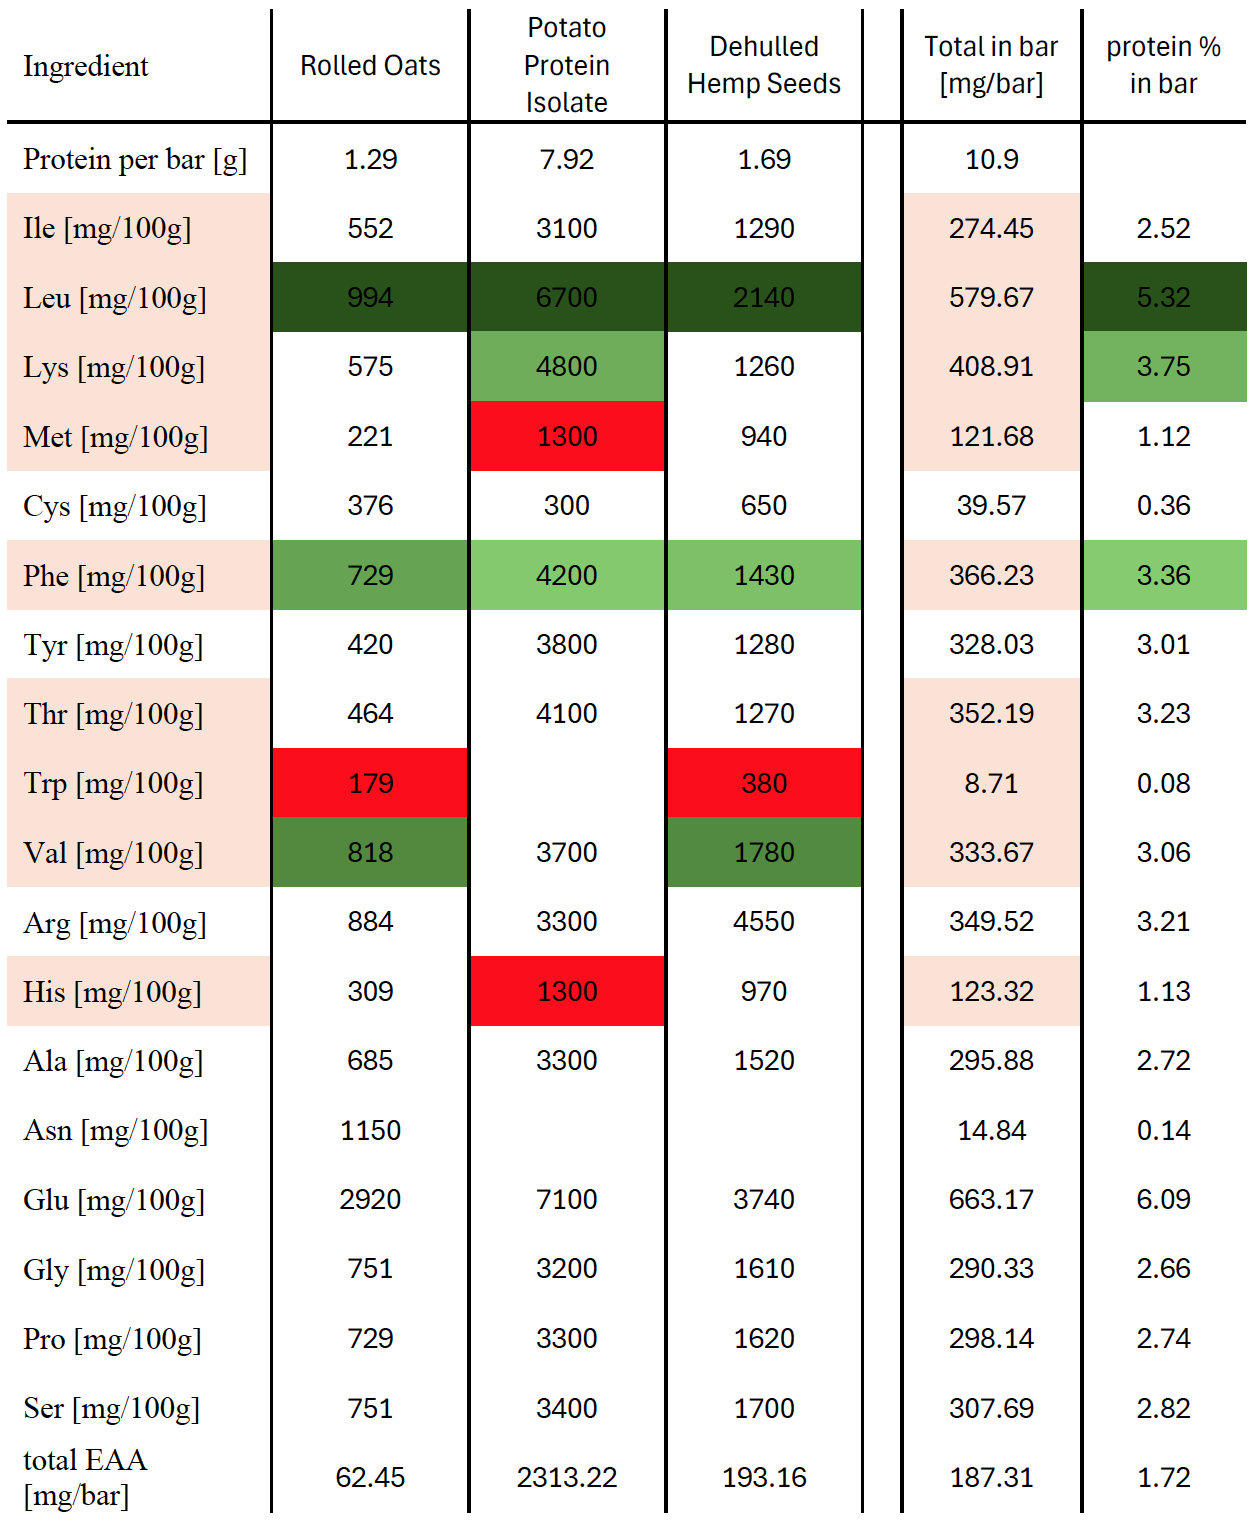
\includegraphics[width=\linewidth]{Figures/tab_amino_acid_01.png}
\end{table}

\vspace{1em}
As shown in Table 6, the main dietary fibre contributors of the hemp seed protein bar are whole hemp seeds, dates (pitted), and rolled oats, who each contributes with 1.32 g, 1.06 g, and 0.99 g, respectively. Processing also influences the dietary fibre profile of the ingredients. In oats, kilning has been used to inactivate lipase enzymes (art\_24), drying dates concentrates their fibre fractions while using whole hemp seeds (un-hulled) preserves their full dietary fibre content. Together, these three ingredients provide the majority of the dietary fibre in the product. When compared with the relative proportions in the product (Table 4), it can be noted, that whole hemp seeds, despite representing only 6.54\% of the bar’s weight, contributes the largest share of the total dietary fibre. Conversely, dates and rolled oats, which consist of 30.84\% and 18.69\% of the bar, respectively, provide less fibre relative to their much larger share of the formulation.

\vspace{1em}
Table 4 contains several blank entries, reflecting that not all ingredients contribute to each of the listed dietary fibre type, and that published data remain scarce, particularly for whole hemp seeds. Nevertheless, it is noteworthy that whole hemp seeds consistently display higher values g/100g for their respective fibre fractions. This highlights the role for whole hemp seeds as the most fibre-dense ingredient and the main contributor to the label “high fibre”. 

\vspace{1em}
The three main ingredients providing dietary fibres, contribute with a diverse palette of fibres. Whole hemp seeds mainly contribute with insoluble fibres such as cellulose, lignin, and hemicellulose. Rolled oats supply cellulose + $\beta-glucan$, lignin, and arabinoxylan, while dates provide these fraction as well as pectin. These fibres differ in solubility and fermentability, thus contributing to a complementary total dietary fibre profile of the hemp seed protein bar (art\_15).

\vspace{1em}
The data used for calculating the fibre fractions for both dates and rolled oats were obtained from published sources given as g/100g dry weight, and g/kg dry weight, respectively. In order to express these values on an as-is basis g/100g, the first step was to make a moisture content correction for the respective ingredients. These conversions were carried out according to Equation 3 and Equation 4, respectively. 


\begin{equation}
    x_{\text{as-is}}\!\left[\frac{\mathrm{g}}{100\,\mathrm{g}}\right]
    = x_{\mathrm{DW}}\!\left[\frac{\mathrm{g}}{100\,\mathrm{g}}\right]\cdot
    \bigl(1 - x_{\text{moisture}}\bigr)
    \label{eq:asis_simple}
\end{equation}

And

\begin{equation}
    x_{\text{as-is}}\!\left[\frac{\mathrm{g}}{100\,\mathrm{g}}\right]
    = \frac{\,x_{\mathrm{DW}}\!\left[\frac{\mathrm{g}}{100\,\mathrm{g}}\right]\,}{10}\,\cdot
    \bigl(1 - x_{\text{moisture}}\bigr)
    \label{eq:asis_div10}
\end{equation}
    
The values for the dietary fibre fractions for whole hemp seeds were given in \% of dry weight, so the calculation had to follow Equation 5.     

\begin{equation}
    x_{\text{as-is}}\!\left[\frac{\mathrm{g}}{100\,\mathrm{g}}\right]
    = \bigl( x_{\mathrm{DW}}\!\left[\tfrac{\mathrm{g}}{100\,\mathrm{g}}\right]
    \cdot (1 - x_{\text{moisture}}) \bigr)
    \cdot x_{\text{DFfraction}}
    \label{eq:asis_dffraction}
\end{equation}

These conversions (Equation 3-5) ensured that all reported values, despite differences in study and unit expression, were standardised to a consistent unit. This enabled a direct comparison between the fibre fractions contributed by the three ingredients. 



\subsubsection{Fatty Acid Profile}
The hemp seed protein bar has a total fat content of 5.84 g. The main contributors to this fat content
are dehulled hemp seeds, whole hemp seeds, and rolled oats, which contribute with 3.38 g, 1.09 g,
and 0.69 g, respectively, as shown in Table 6. Processing steps also affect the lipid quality.

\vspace{1em}
Processing steps also affect the lipid quality. Dehulling the hemp seeds increases the fat fraction by removing the hull mass. For a deeper insight into the specific fatty acid profile of the hemp protein bar, Table 5 was constructed to illustrate the distribution of fatty acid fractions from the top three ingredients. 

\begin{table}[H]
    \centering
    \caption{Contribution of the main dietary fibre sources (dates, rolled oats, and whole hemp seeds) to the hemp seed protein bar,
    expressed as total dietary fibre per bar and distribution of fibre fractions. Coloured cells indicate relative contribution, with light
    green representing lowest top three value and dark green representing the highest of the top three. The red coloured cells indicate the
    lowest value for each ingredient.}
    \label{tab:df_tab_01}
    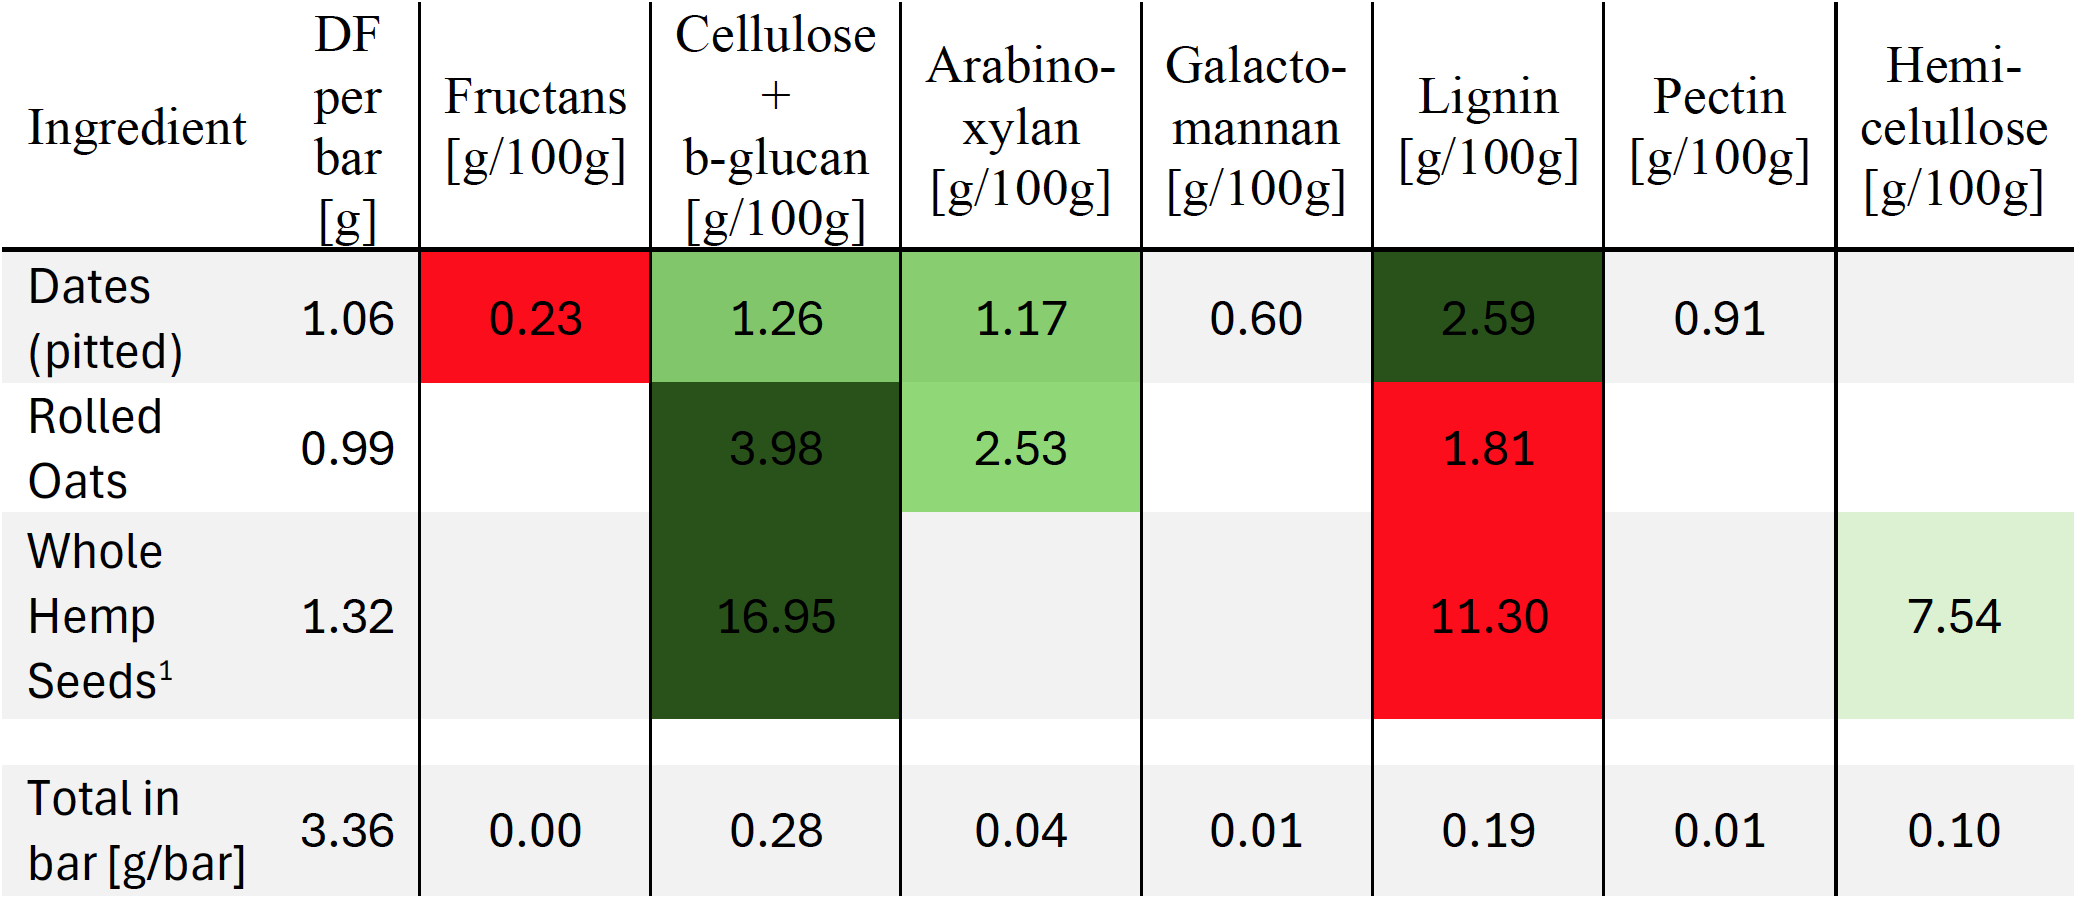
\includegraphics[width=\linewidth]{Figures/tab_df_01.png}
\end{table}

\vspace{1em}
It can be seen in Table 5, that the fatty acid profile is dominated by the polyunsaturated fatty acids (PUFAs). Notably, linoleic acid (LA, C18:2 n-6) and $\alpha$-linoleic acid (ALA, C18:3 n-3) constitutes 69.47\% of the total fatty acids quantified in the bar. These two essential fatty acids, LA (an omega-6) and ALA (an omega-3), cannot be synthetised by the human body and must therefore be obtained through diet. The abundance in the fatty acid profile highlights the nutritional value of the hemp protein bar. Previous studies have reported that LA and ALA from hemp seeds may the nervous system, supporting the health of blood vessels and to protect against cardiovascular diseases (art\_21). 

\vspace{1em}
Omega-6 tends to have pro-inflammatory pathways, whereas omega-3 supports anti-inflammatory responses. Therefore, maintaining an appropriate balance between these fatty acids is imperative (art\_21). Although EFSA does not prescribe a fixed omega-6 to omega-3 ratio, its Adequate Intake levels for LA (4\% of energy) and ALA (0.5\% of energy) imply a target ratio of approximately 3\:1. The hemp protein bar provides 1.022 g of omega-6 and 0.430 g of omega-3, yielding a ratio of 2.38\:1, close to, but slightly below the recommended guidelines (art\_22). 

\vspace{1em}
As stated, EFSA has set the Adequate Intake levels for LA and ALA to 4E\% and 0.5E\%, respectively. Based on a diet of 2000 kcal, this corresponds to approximately 8.9 g/day of LA and 1.1 g/day of ALA. 



\vspace{1em}
The hemp protein bar will provide roughly 11.5\% and 39\% of the daily requirements of LA and ALA, respectively. Although the substantial contribution to the daily fatty acid intake, these levels does not meet the conditions set by EU for nutrition and health claims. ALA falls below the $geq$ 0.3 g/100kcal threshold for the claim “source of omega-3 fatty acids” (art\_23), and LA remains below the $\geq$ 1.5 g/100kcal threshold requires for the claim “contributes to the maintenance of normal blood cholesterol levels” (art\_24).

\vspace{1em}
Saturated fatty acids (SFAs) in the hemp protein bar sum to 0.277g per bar, or 13.27\% of the total fatty acid profile. Palmitic acid (C16:0) is the predominant fraction, contributing with 0.199 g per bar. 
Monounsaturated fatty acids (MUFAs) account for 0.360 g of the hemp bar, representing 17.24\% of the 2.09 g total fatty acids. Table 5 illustrates that oleic acid (C18:1, n-9) is the dominant MUFA, consistently ranking among the three most abundant fatty acid fractions in dehulled hemp seeds, whole hemp seeds, and rolled oats. 


\begin{table}[H]
    \centering
    \caption{Contribution of the main dietary fibre sources (dates, rolled oats, and whole hemp seeds) to the hemp seed protein bar,
    expressed as total dietary fibre per bar and distribution of fibre fractions. Coloured cells indicate relative contribution, with light
    green representing lowest top three value and dark green representing the highest of the top three. The red coloured cells indicate the
    lowest value for each ingredient.}
    \label{tab:fatty_acid_tab_01}
    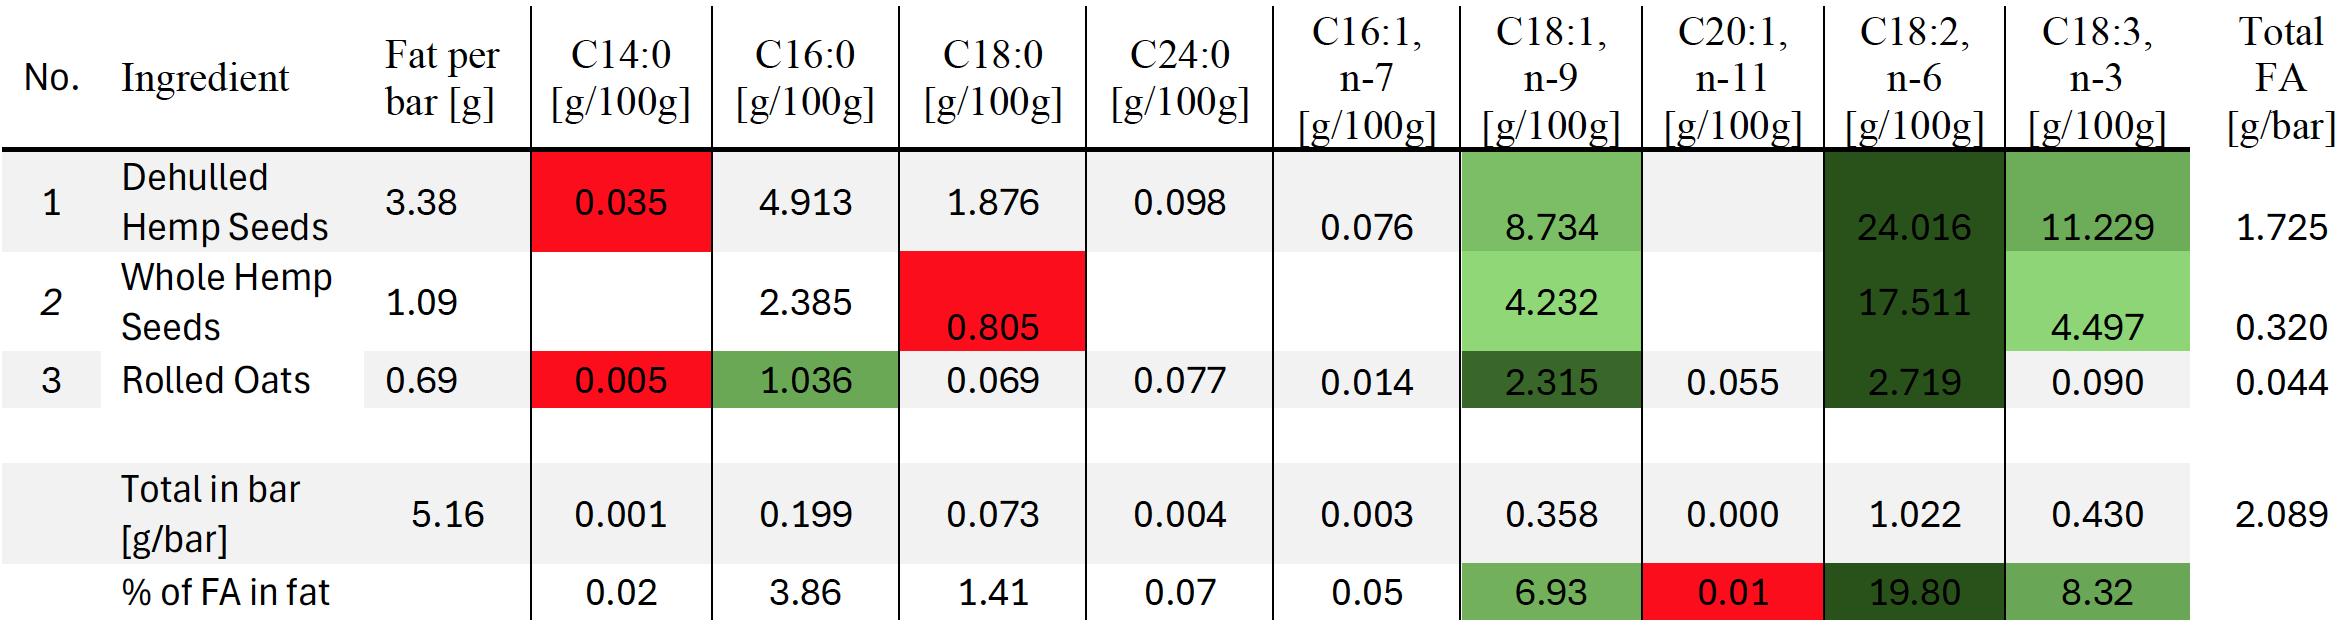
\includegraphics[angle=90,origin=c,width=0.23\textheight]{Figures/tab_fatty_01.png}
\end{table}





\printbibliography

% \begin{appendices}
%     \chapter{Appendix}
\section{Appendix 1 - Principles for isolation of microorganisms form fermented food and beverages}
\label{appendix1}
%\includepdf[pages=-]{Appendices/Isolation101.pdf}

% \end{appendices}

\end{document}